\documentclass[../main.tex]{subfiles}
\graphicspath{{\subfix{../images/}}}
\begin{document}

\chapter{System Analysis and Design}
\section{System architecture}

The game will run on the unity game engine utilising a lot of its features. As for the simulation of the circuits the we will use the C\# library SpiceSharp. SpiceSharp is a circuits simulation library that is compatible with the Berkeley Spice simulator. The player will interact with the game through its user interface, those interactions could be navigational interactions to transition from one menu or scene to another, or they could be gameplay interactions when playing a level. Then in order to complete a level the player needs to achieve some goals that are introduced at the beginning of the level. The circuits submitted by the player is then simulated using SpiceSharp and the results are sent back to the game, the game then decides whether the goals were achieved or not.
\begin{figure}[ht]
\centering
\includegraphics[scale=0.14]{images/chapter3/System Design & Architecture.png}
\caption{System Design \& Architecture.png}
\label{System Design and  Architecture.png}
\end{figure}

\section{System analysis}

\subsection{Context Diagram}
\begin{figure}[ht]
\centering
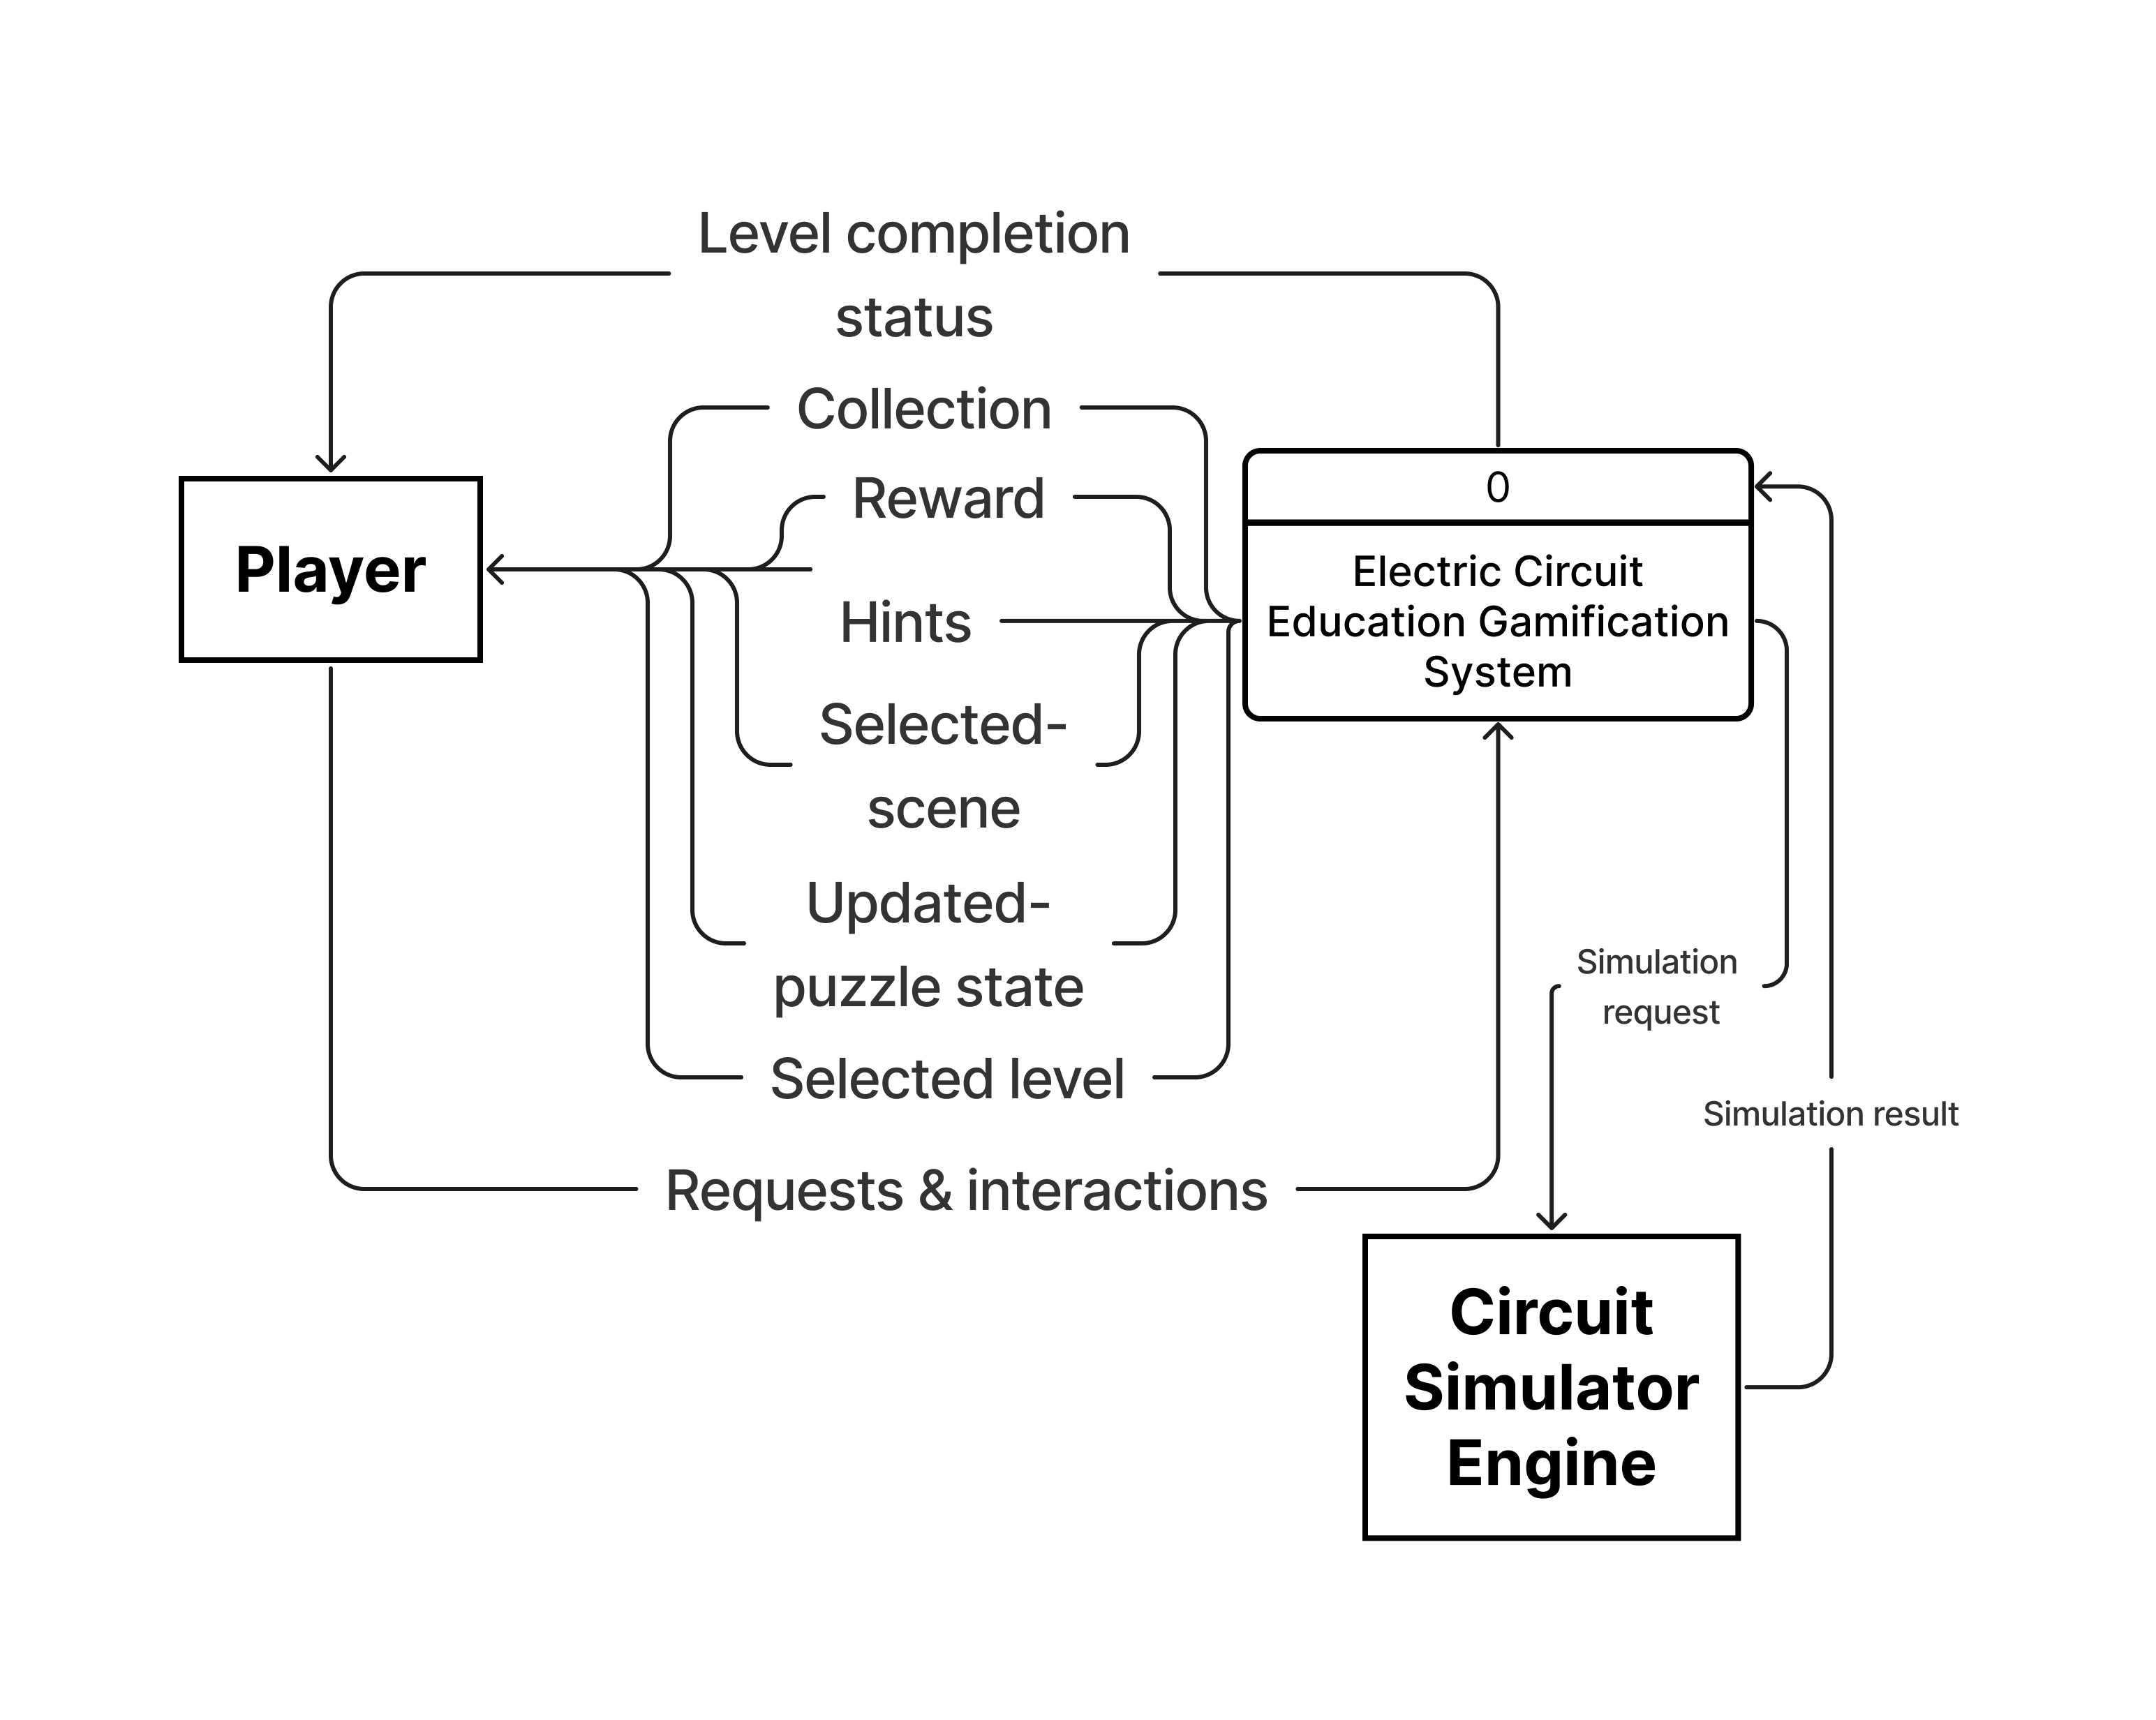
\includegraphics[scale=0.3]{images/chapter3/Context.png}
\caption{Context Diagram}
\label{Context.png}
\end{figure}
\vfill

\newpage
\subsection{Process Diagram}
\begin{figure}[ht!]
\centering
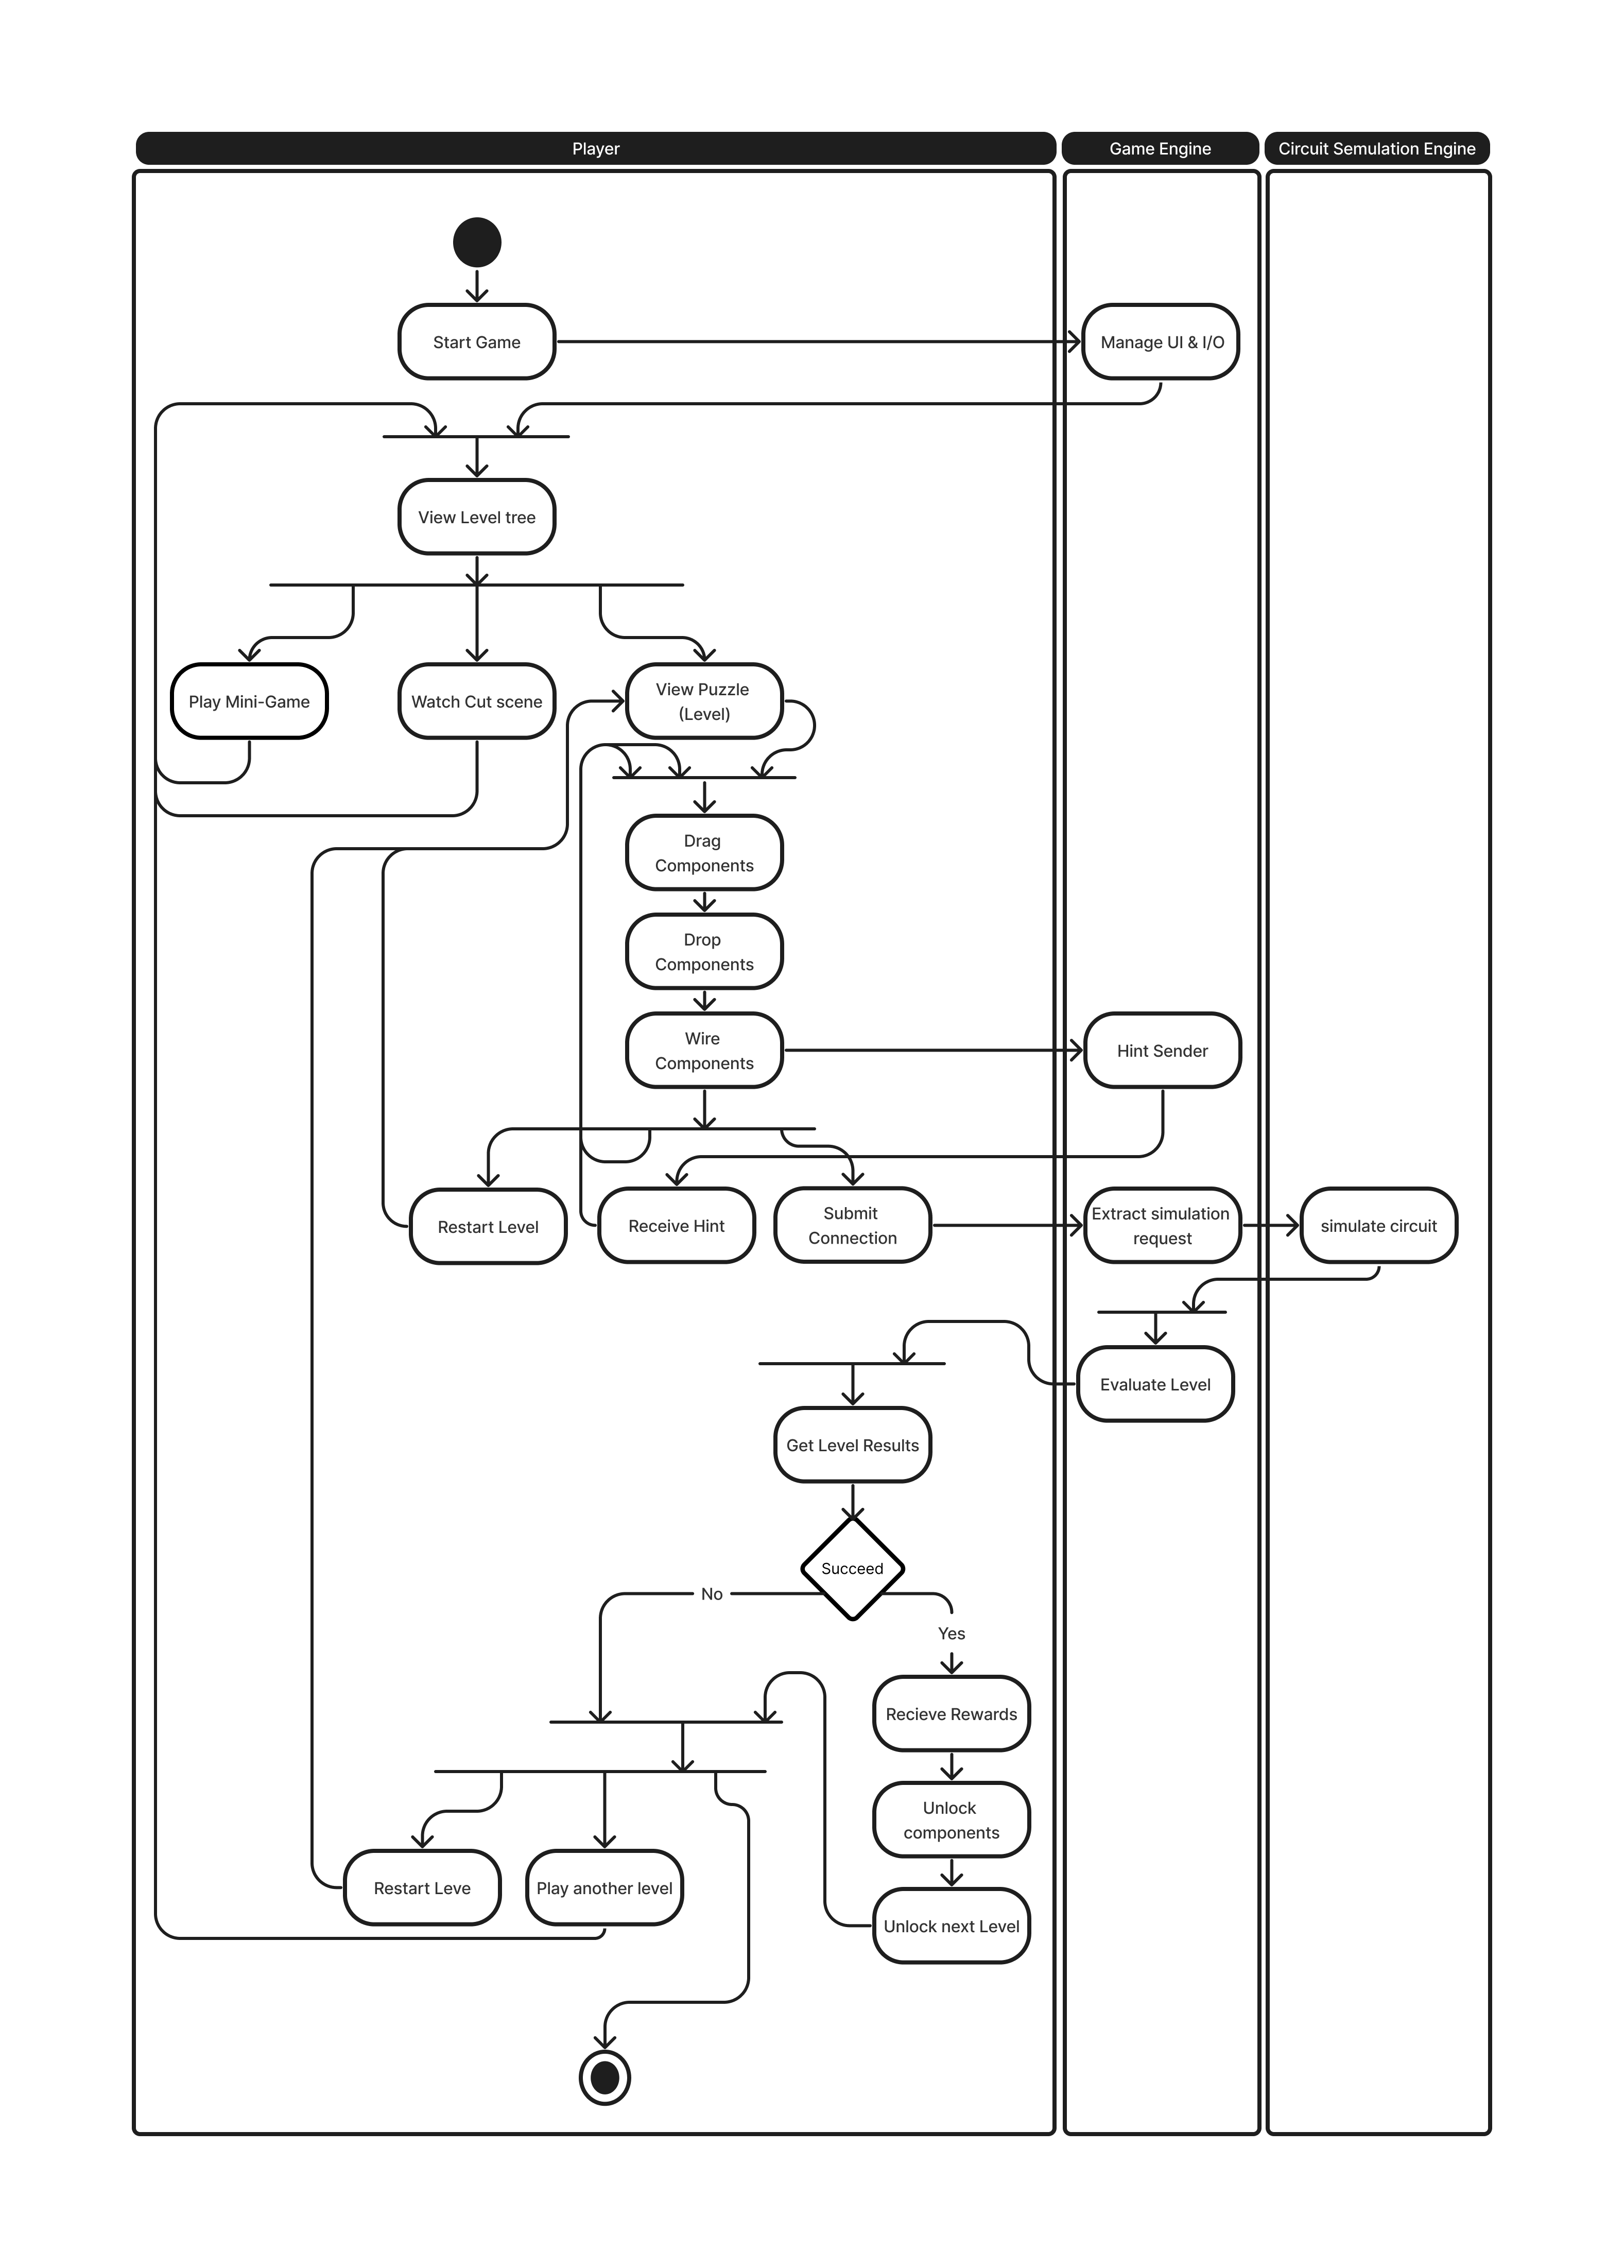
\includegraphics[scale=0.27]{images/chapter3/Process.png}
\caption{Process Diagram}
\label{prcess.png}
\end{figure}
\vfill

\newpage
\subsection{Use Case Diagram}
\vfill
\begin{figure}[!ht]
\centering
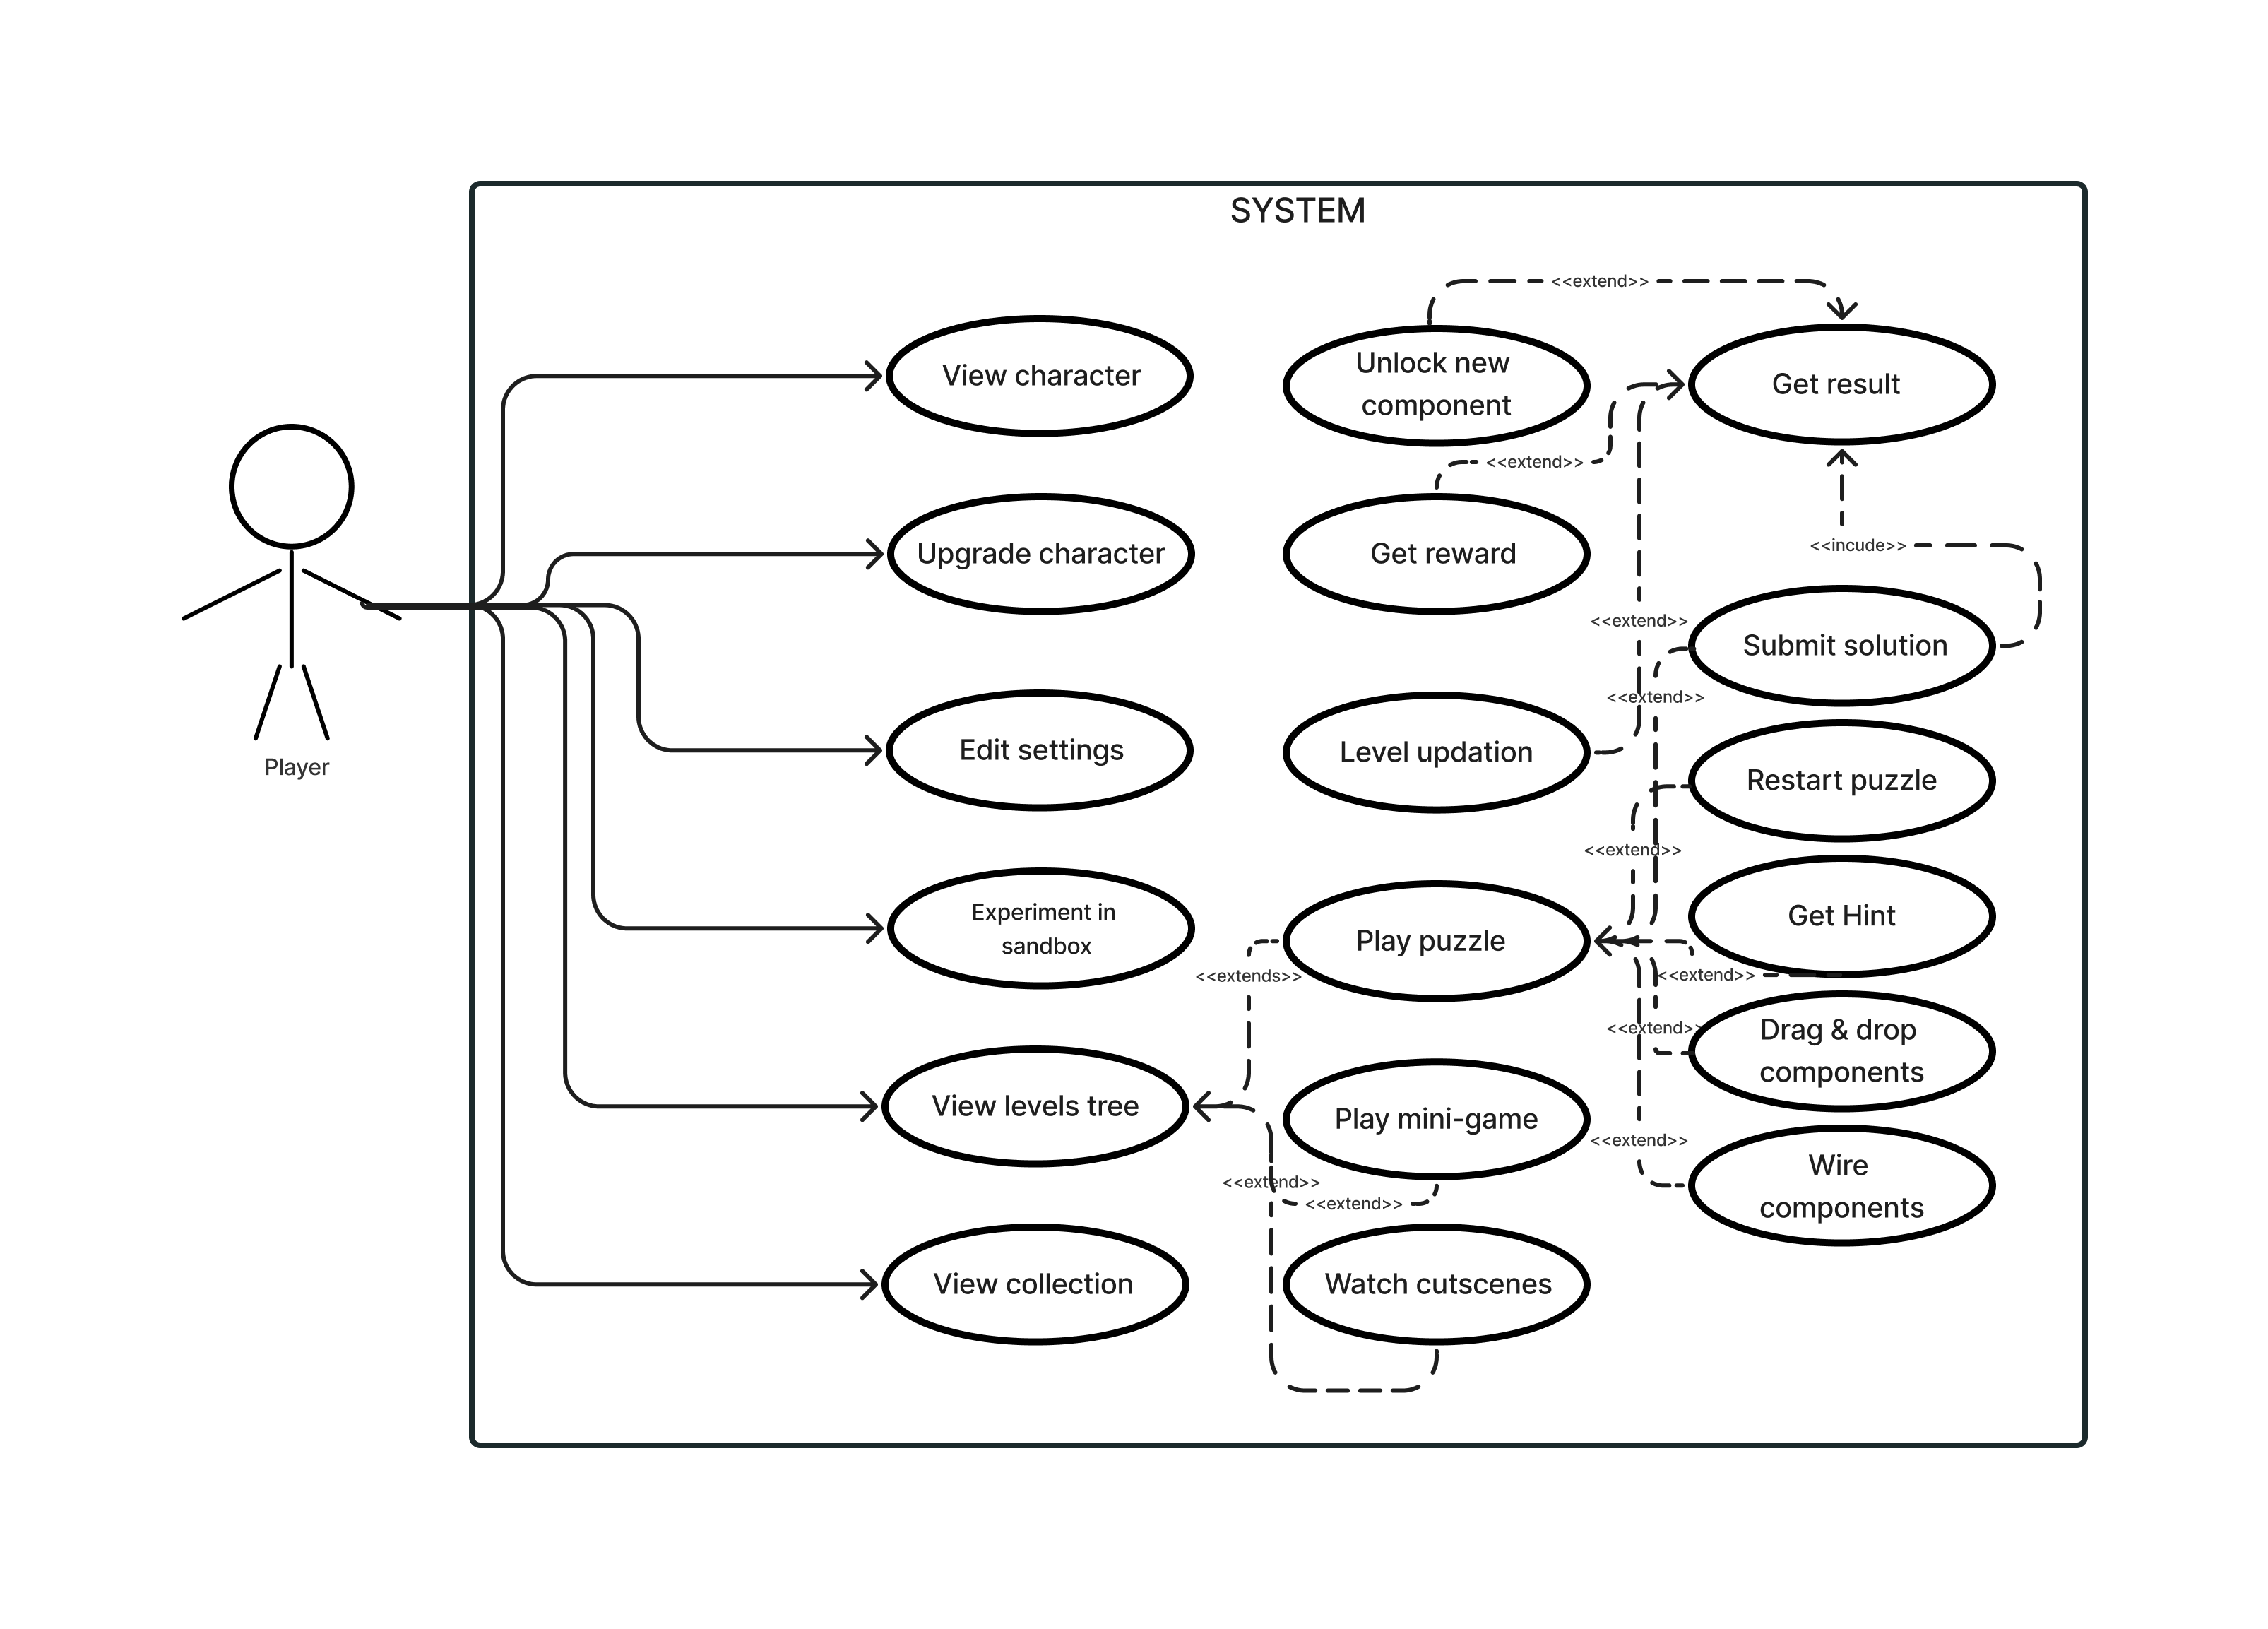
\includegraphics[scale=0.27]{images/chapter3/Usecase.png}
\caption{Usecase Diagram}
\label{Use Case.png}
\end{figure}
\vfill
\newpage
\subsection{Data-Flow Diagram}
\begin{figure}[ht!]
\centering
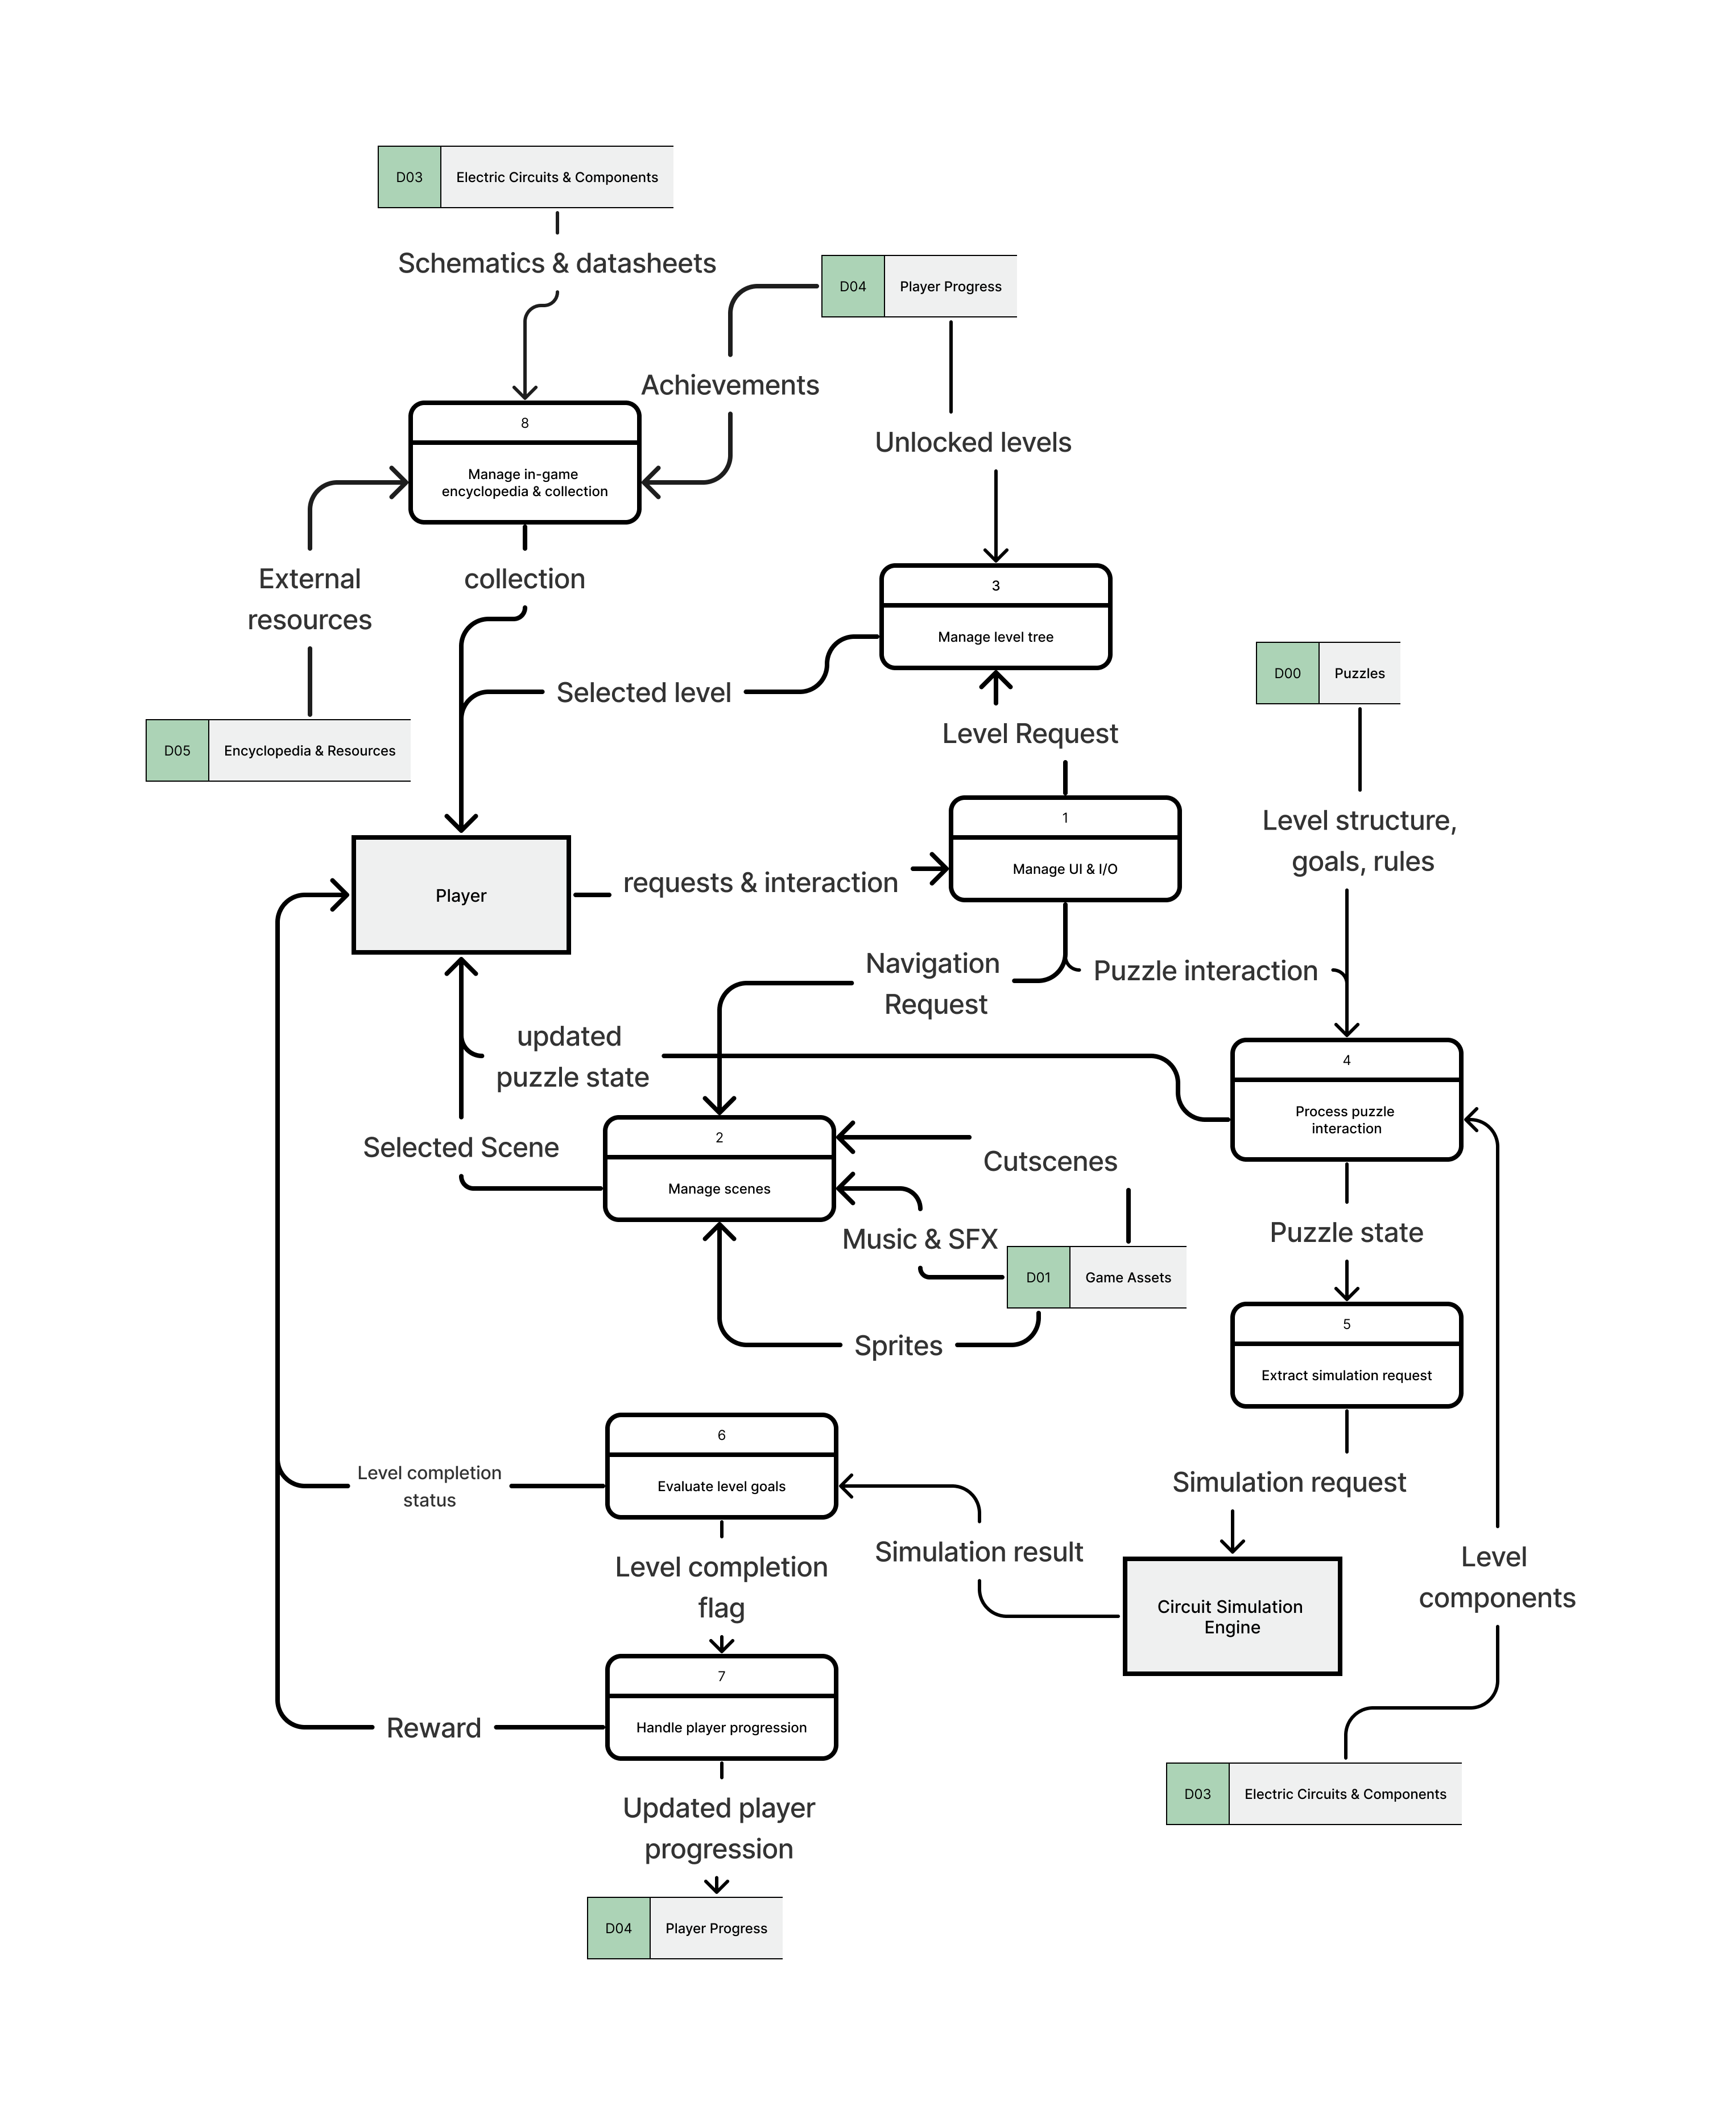
\includegraphics[scale=0.3]{images/chapter3/DFD.png}
\caption{Data-Flow Diagram}
\label{Data-Flow Diagram}
\end{figure}
\vfill
\newpage
\subsection{Sequence Diagram}
\begin{figure}[h!t]
\centering
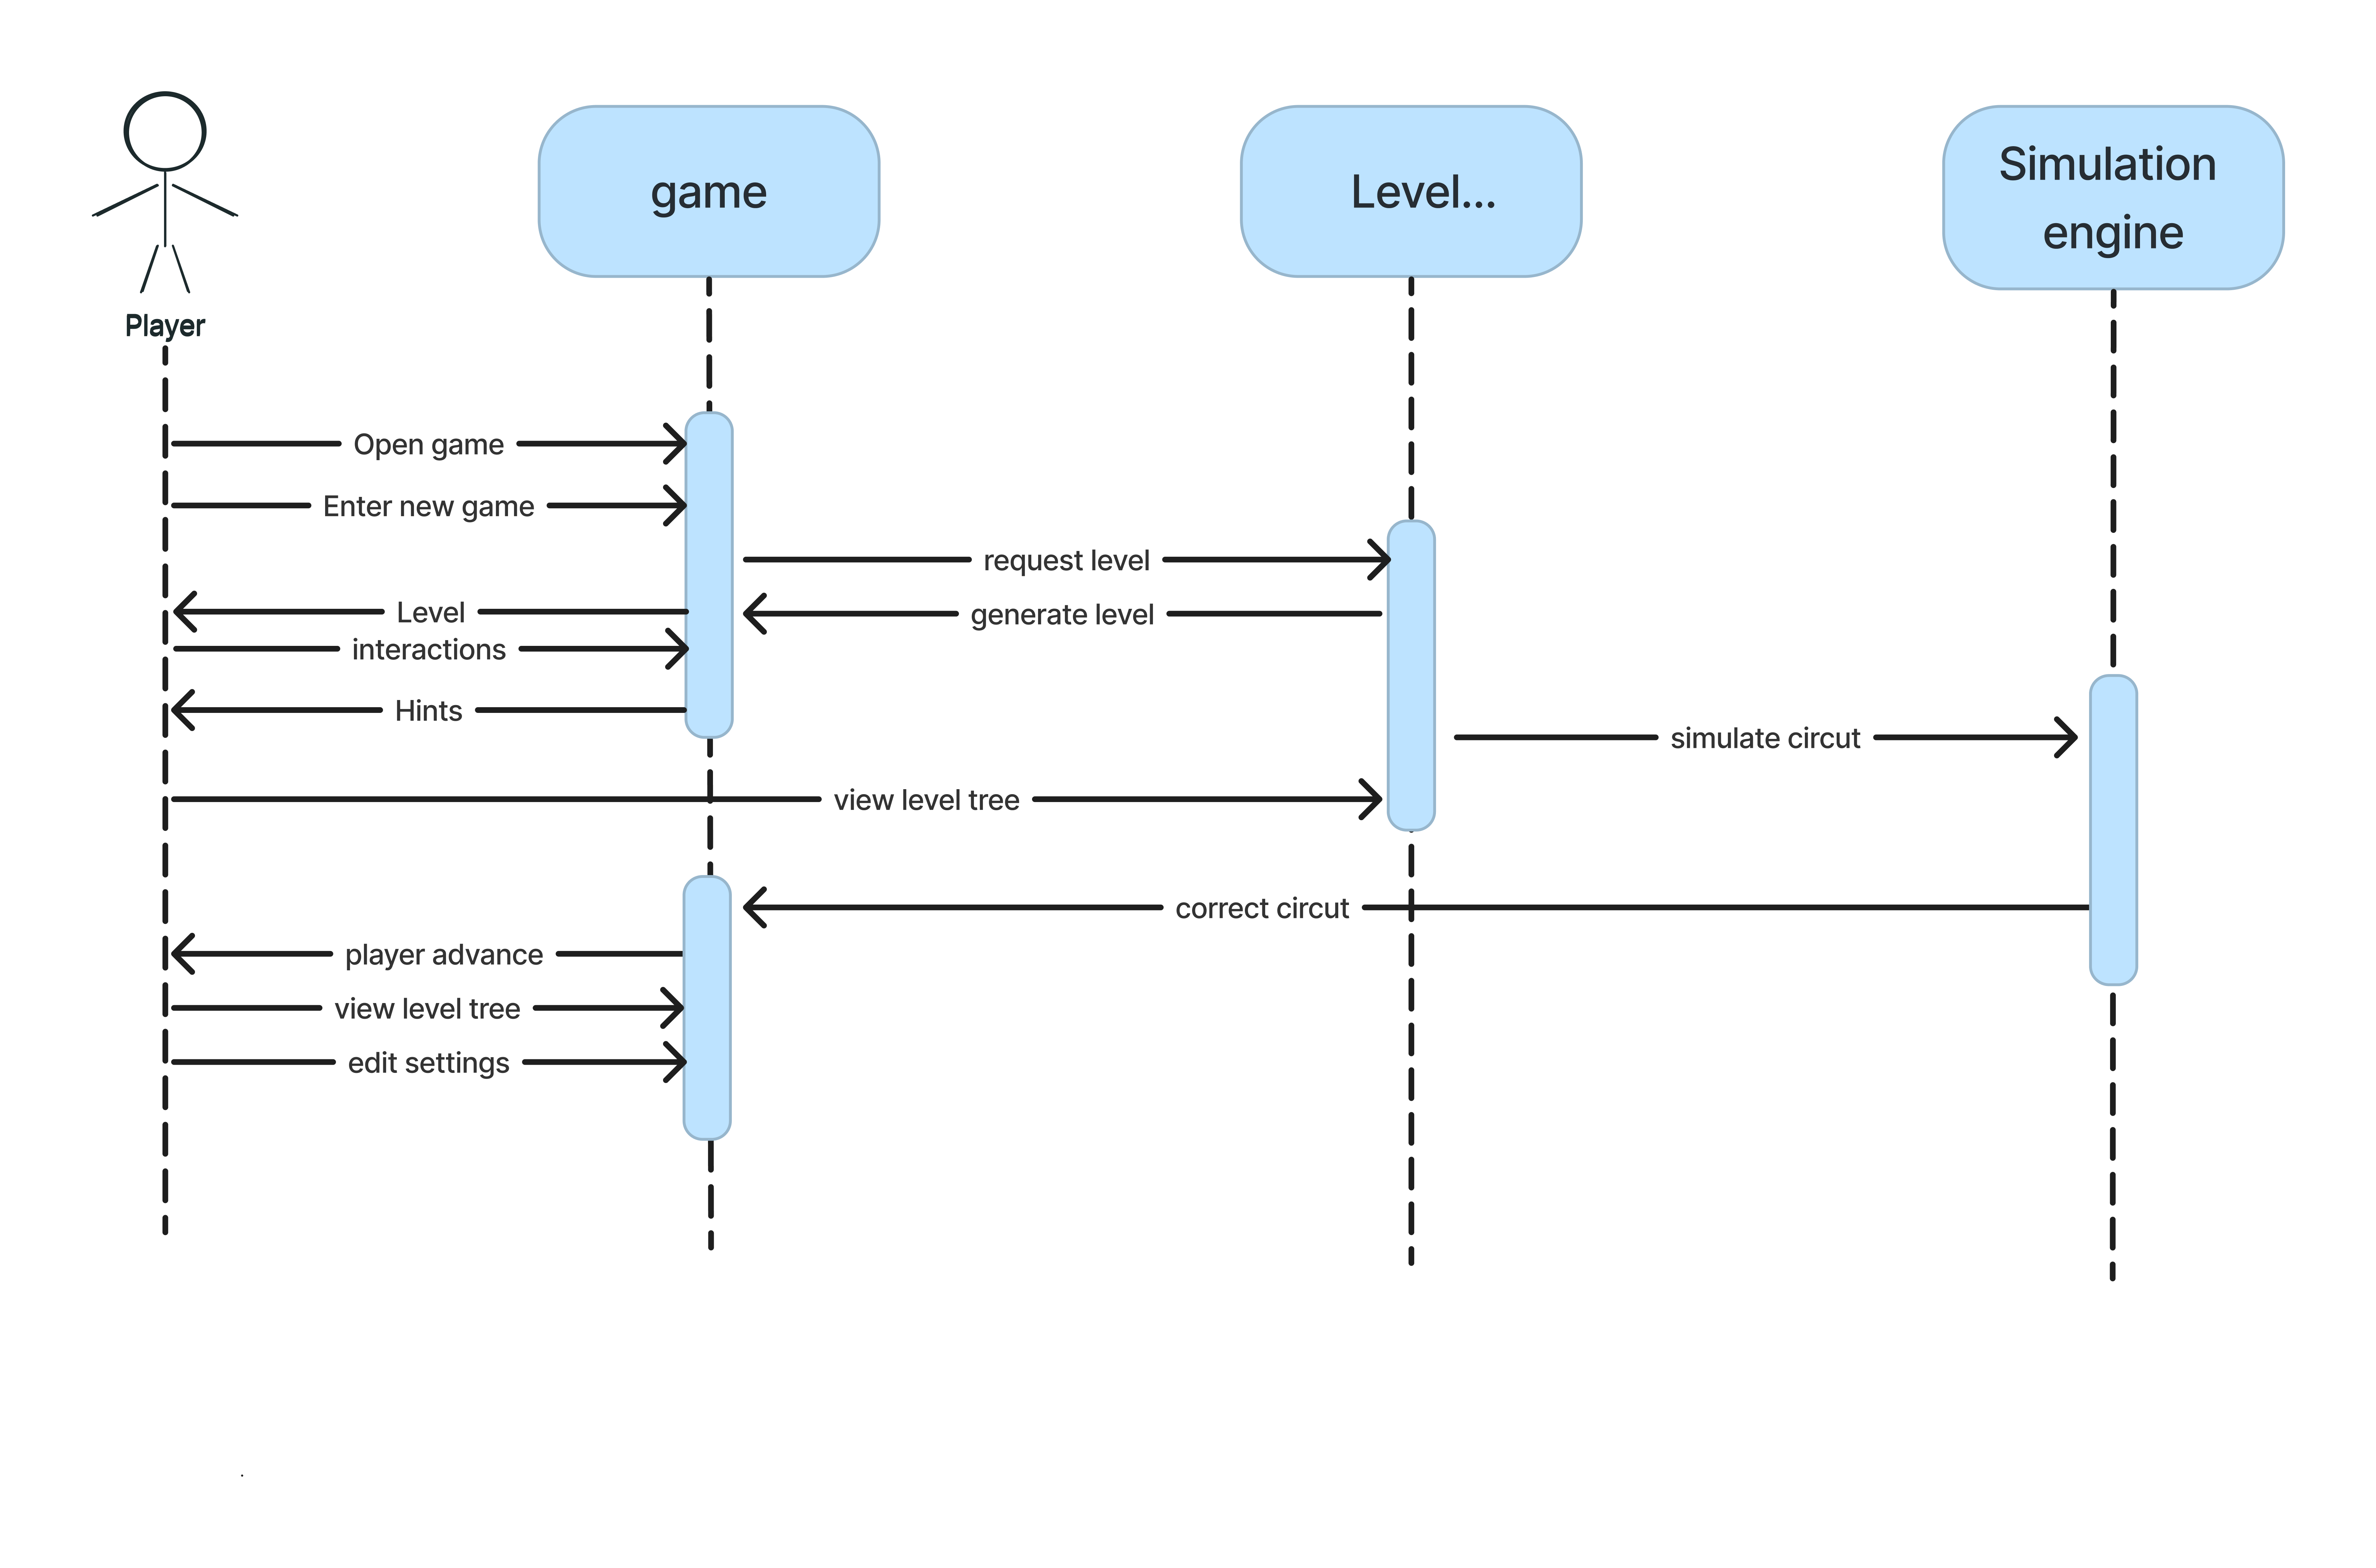
\includegraphics[scale=0.11]{images/chapter3/sq.png}
\caption{Sequence Diagram}
\label{Sequence Diagram}
\end{figure}
\vfill
\newpage
\subsection{Class Diagram}

\subsubsection{Simulator and Simulation Manager}

\begin{figure}[h!t]
\centering
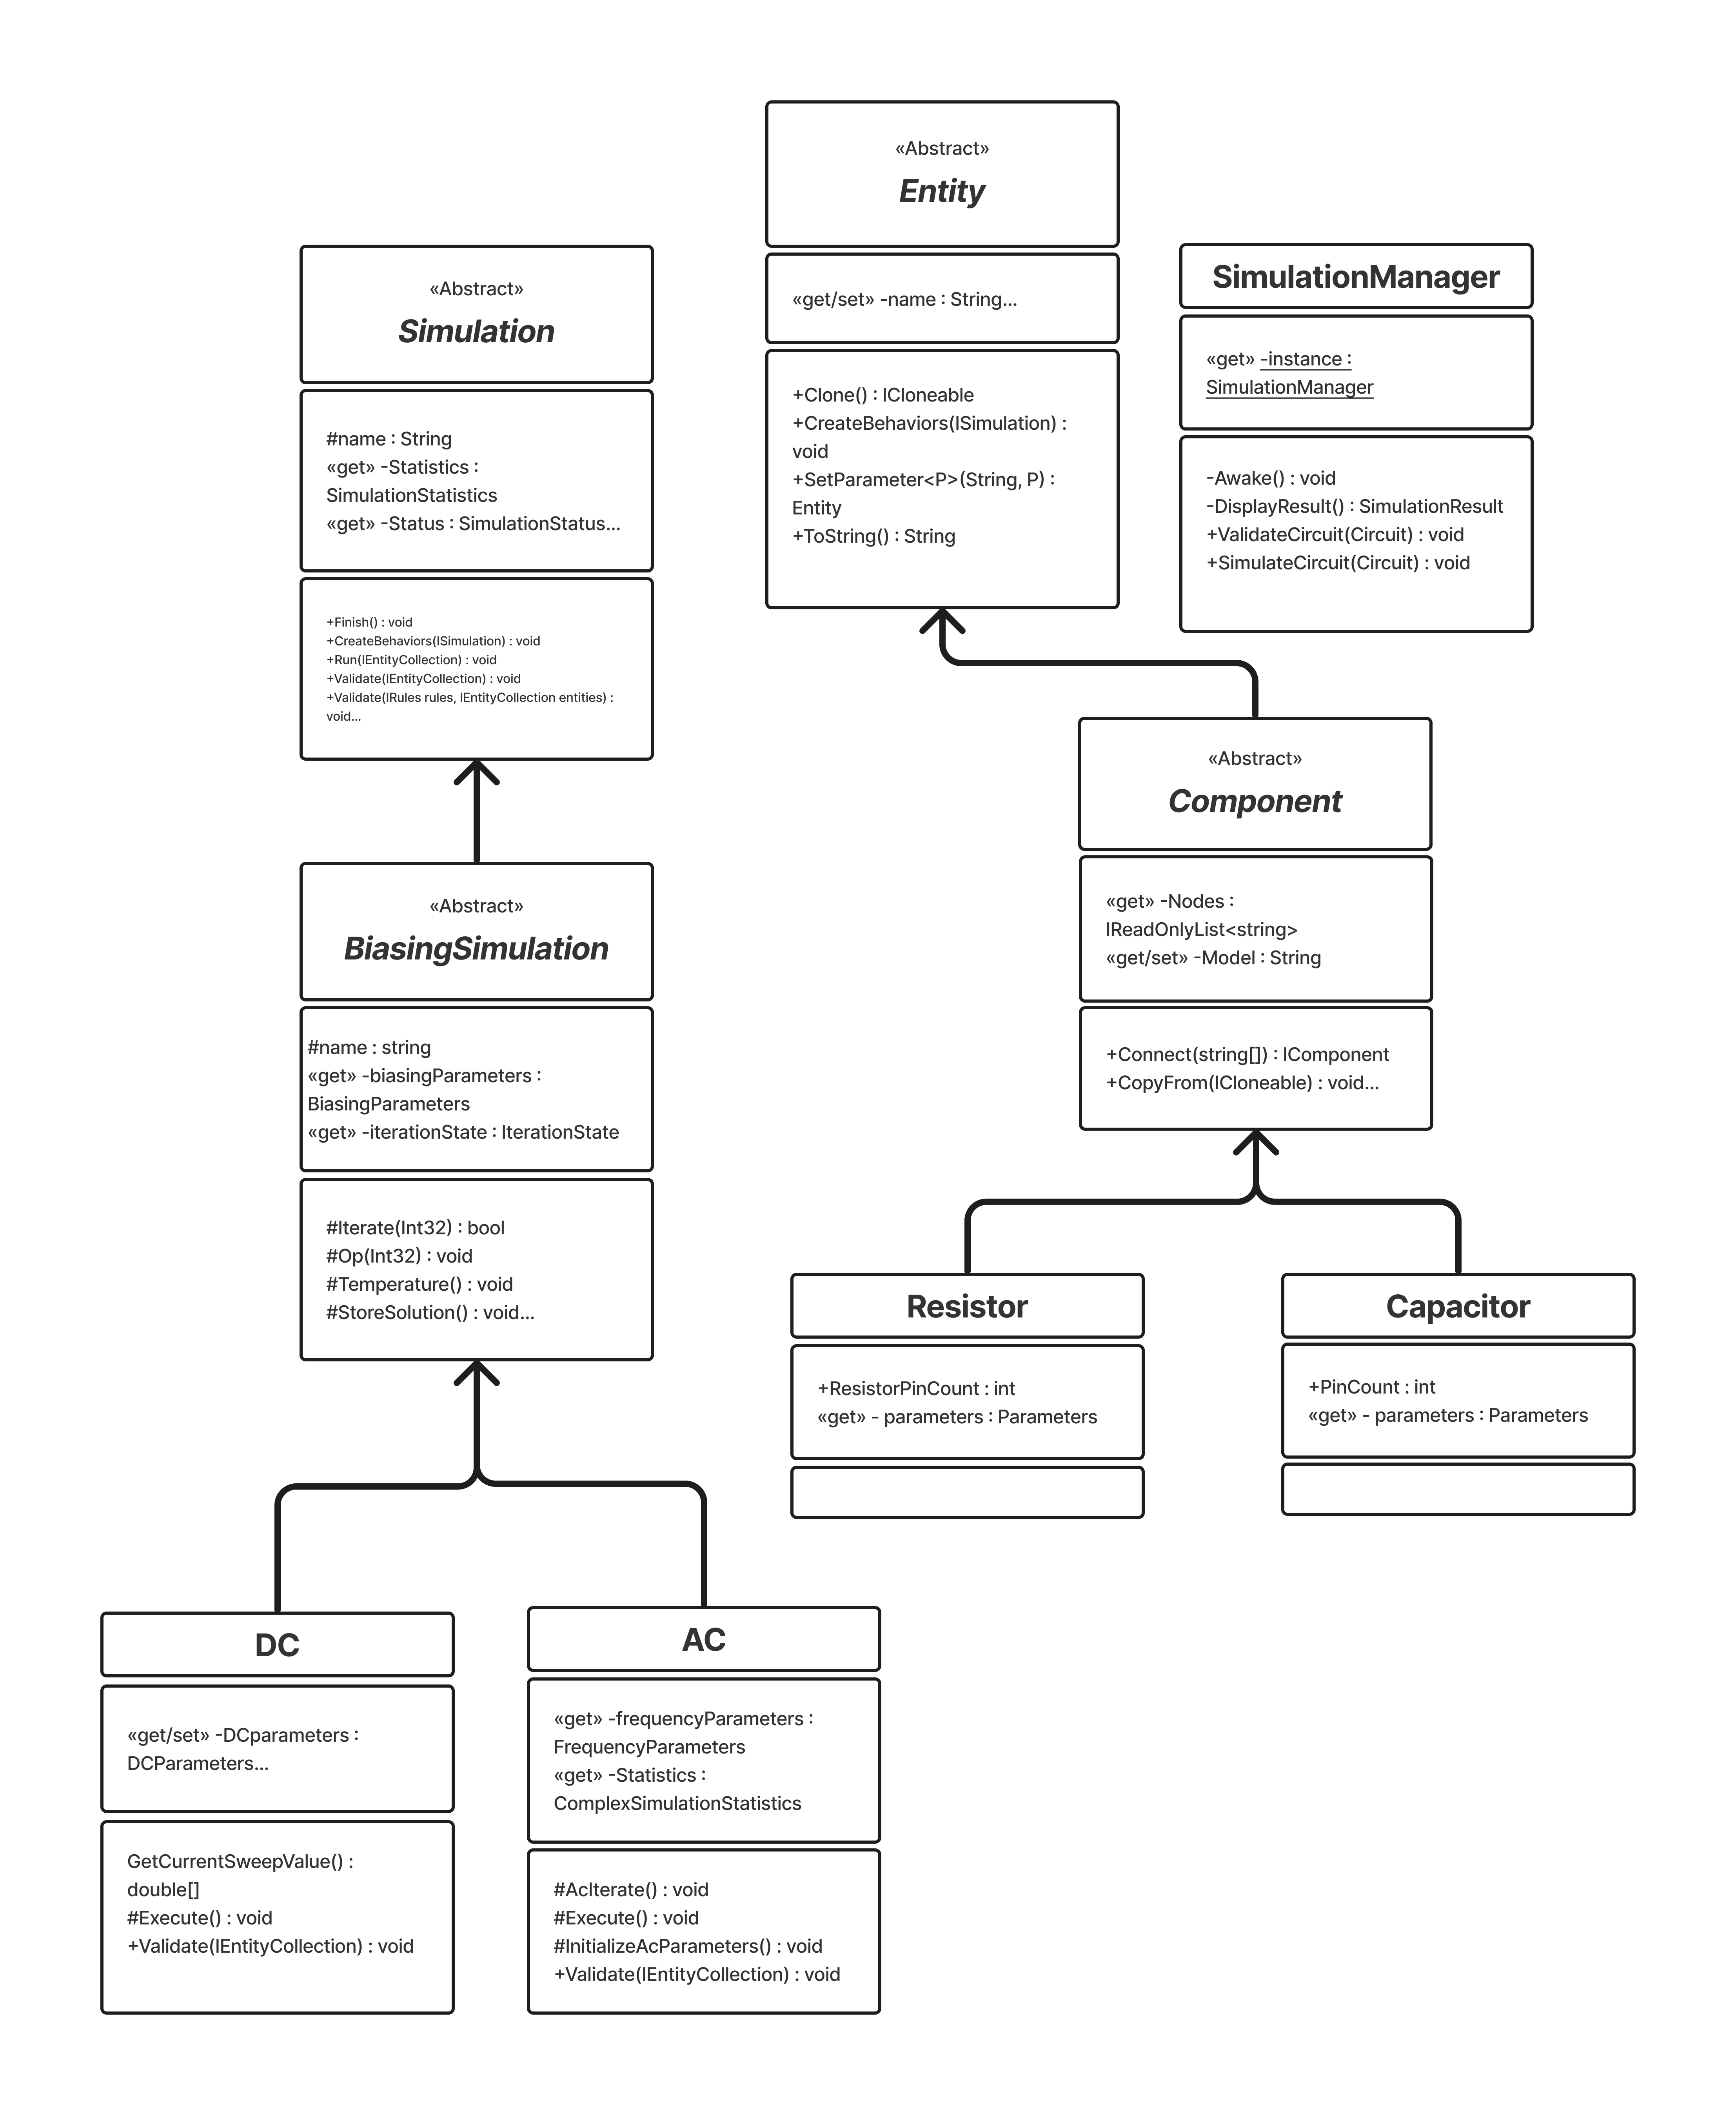
\includegraphics[scale=0.2]{images/chapter3/Class1.png}
\caption{Simulator and Simulation Manager Class Diagram}
\label{Simulator and Simulation Manager}
\end{figure}

\subsubsection{GameComponents and ComponentManager}

\begin{figure}[h!t]
\centering
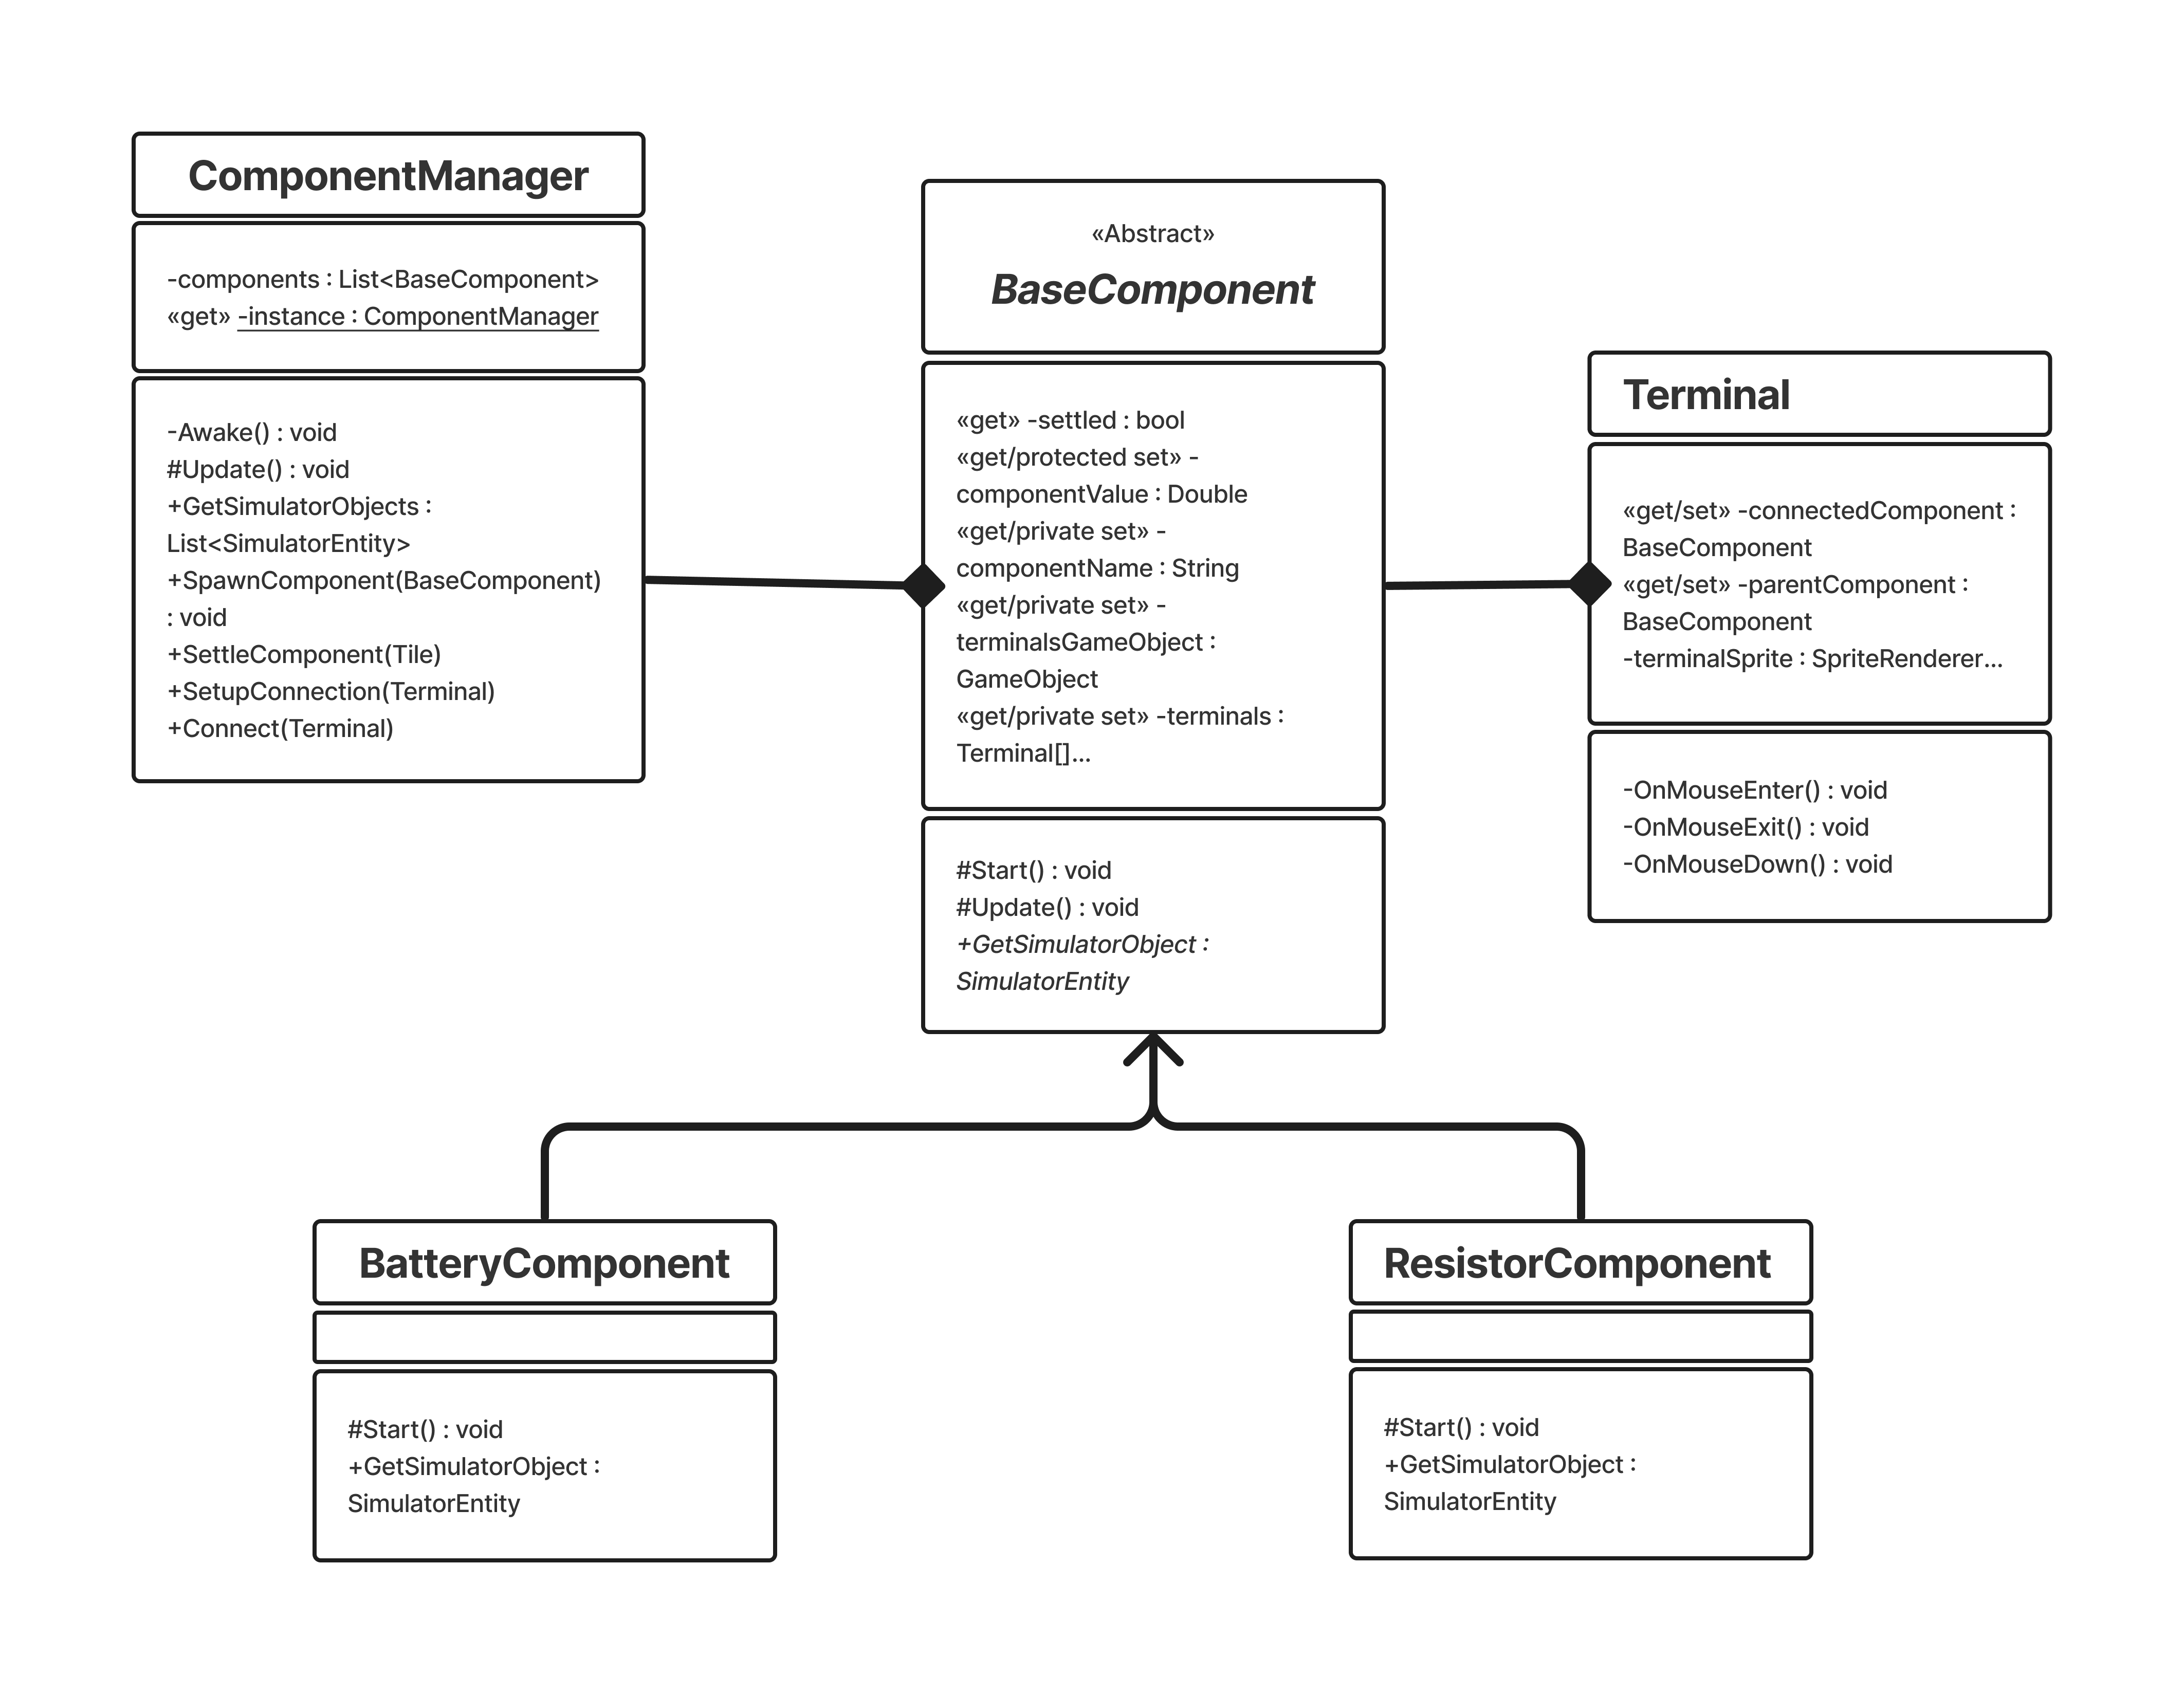
\includegraphics[scale=0.2]{images/chapter3/Class2.png}
\caption{GameComponents and ComponentManager Class Diagram}
\label{GameComponents and ComponentManager }
\end{figure}
\newpage
\subsubsection{GameManager}\begin{figure}[h!]
\centering
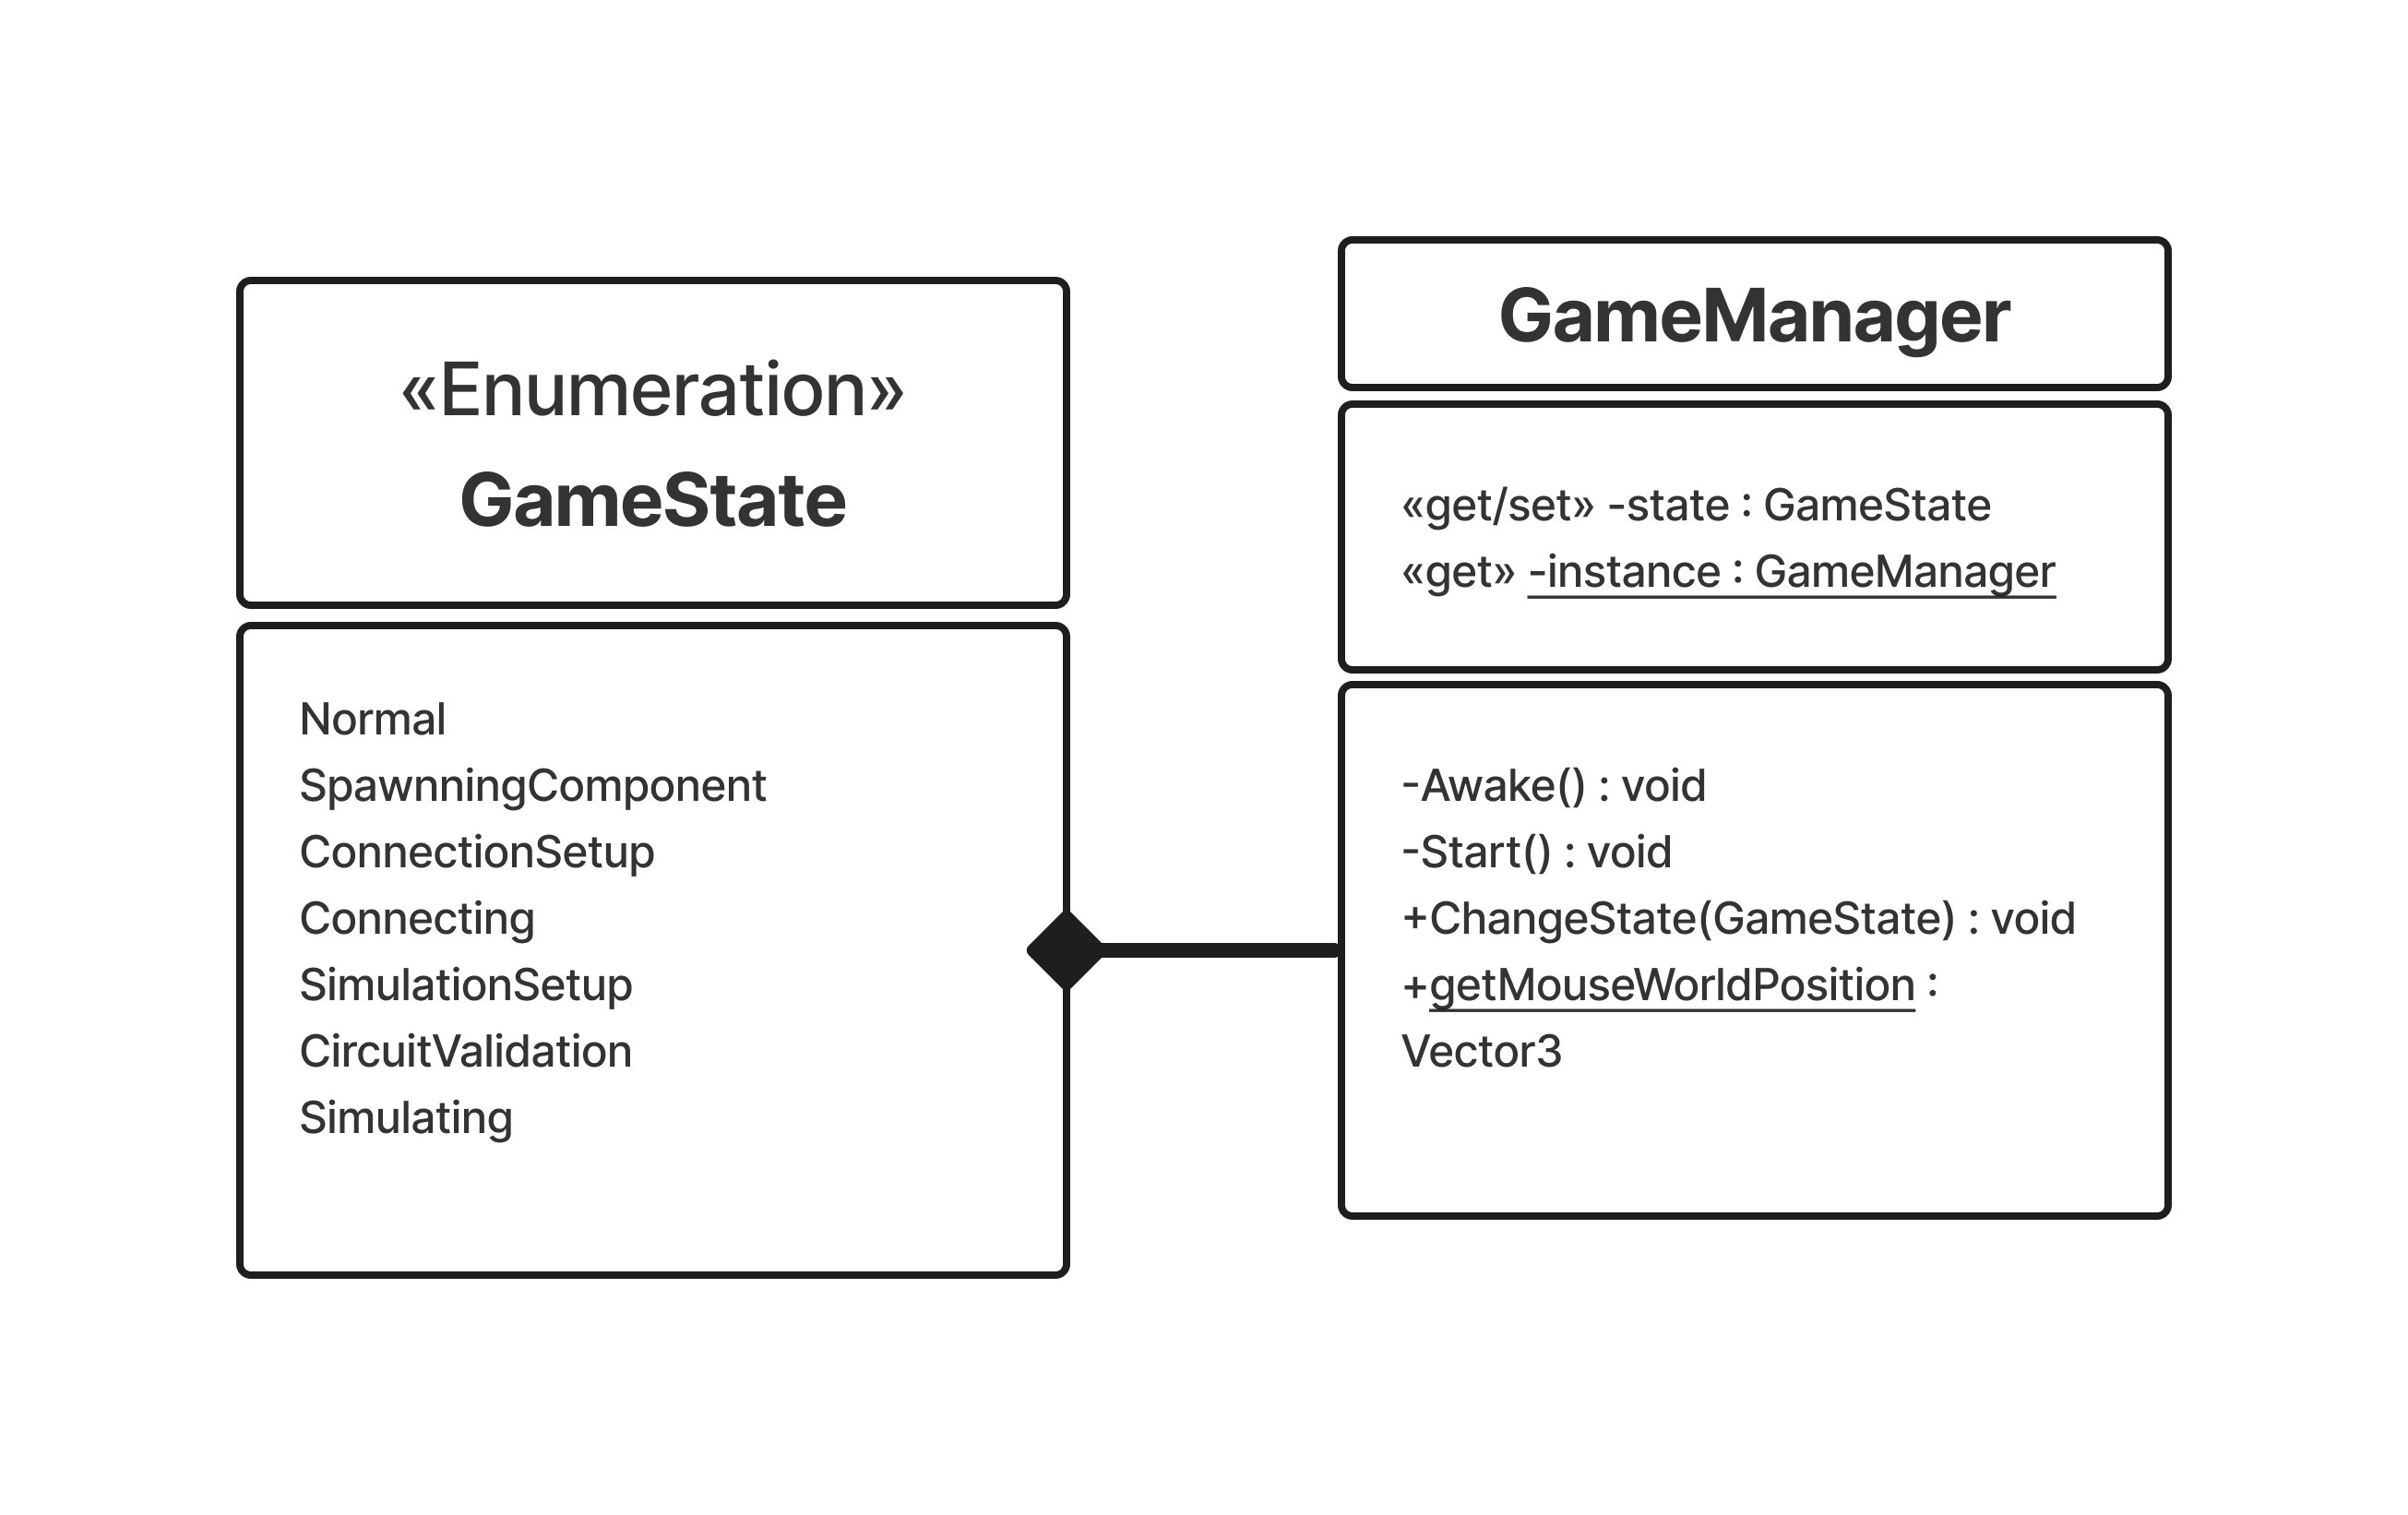
\includegraphics[scale=0.3]{images/chapter3/Class3.png}
\caption{GameManager Class Diagram}
\label{GameManager }
\end{figure}
\vfill
\newpage
\subsection{Entity Relation Diagram }
\begin{figure}[h!]
\centering
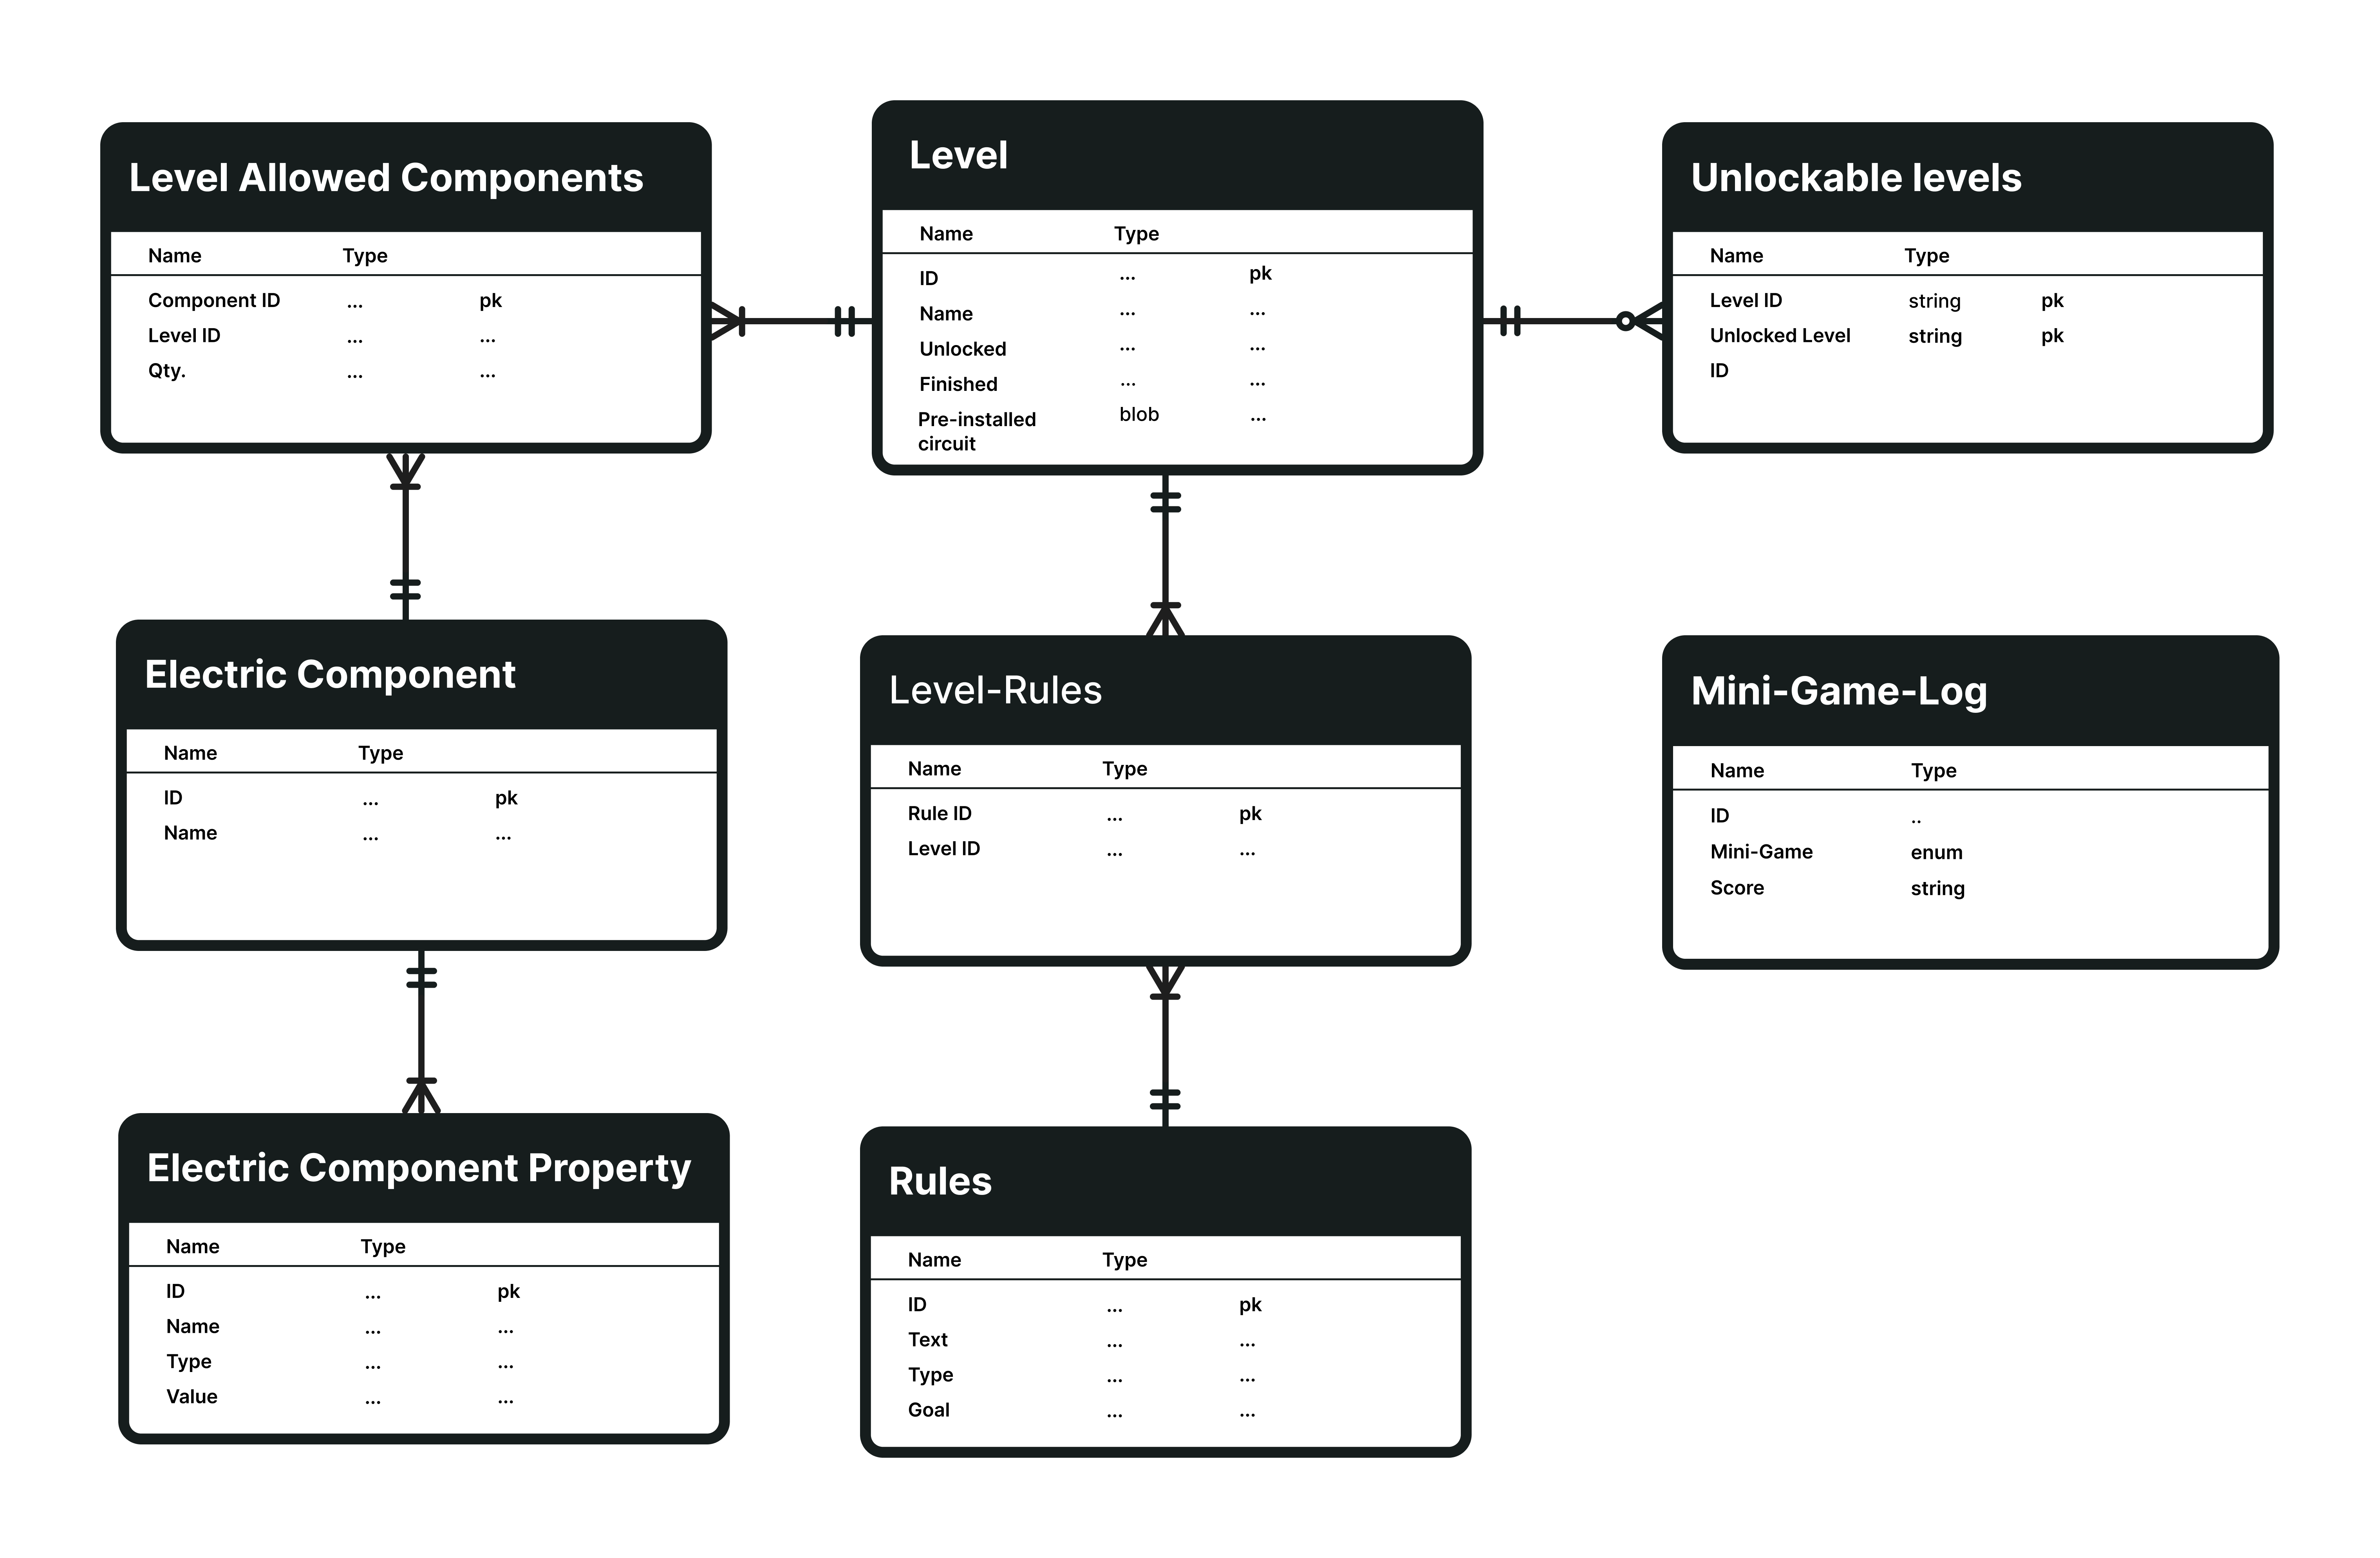
\includegraphics[scale=0.15]{images/chapter3/ERD.png}
\caption{Entity Relation Diagram }
\label{Entity Relation Diagram }
\end{figure}
\vfill
\newpage

\subsection{State Chart Diagram}
\subsubsection{Drag and drop components}

\begin{figure}[h!]
\centering
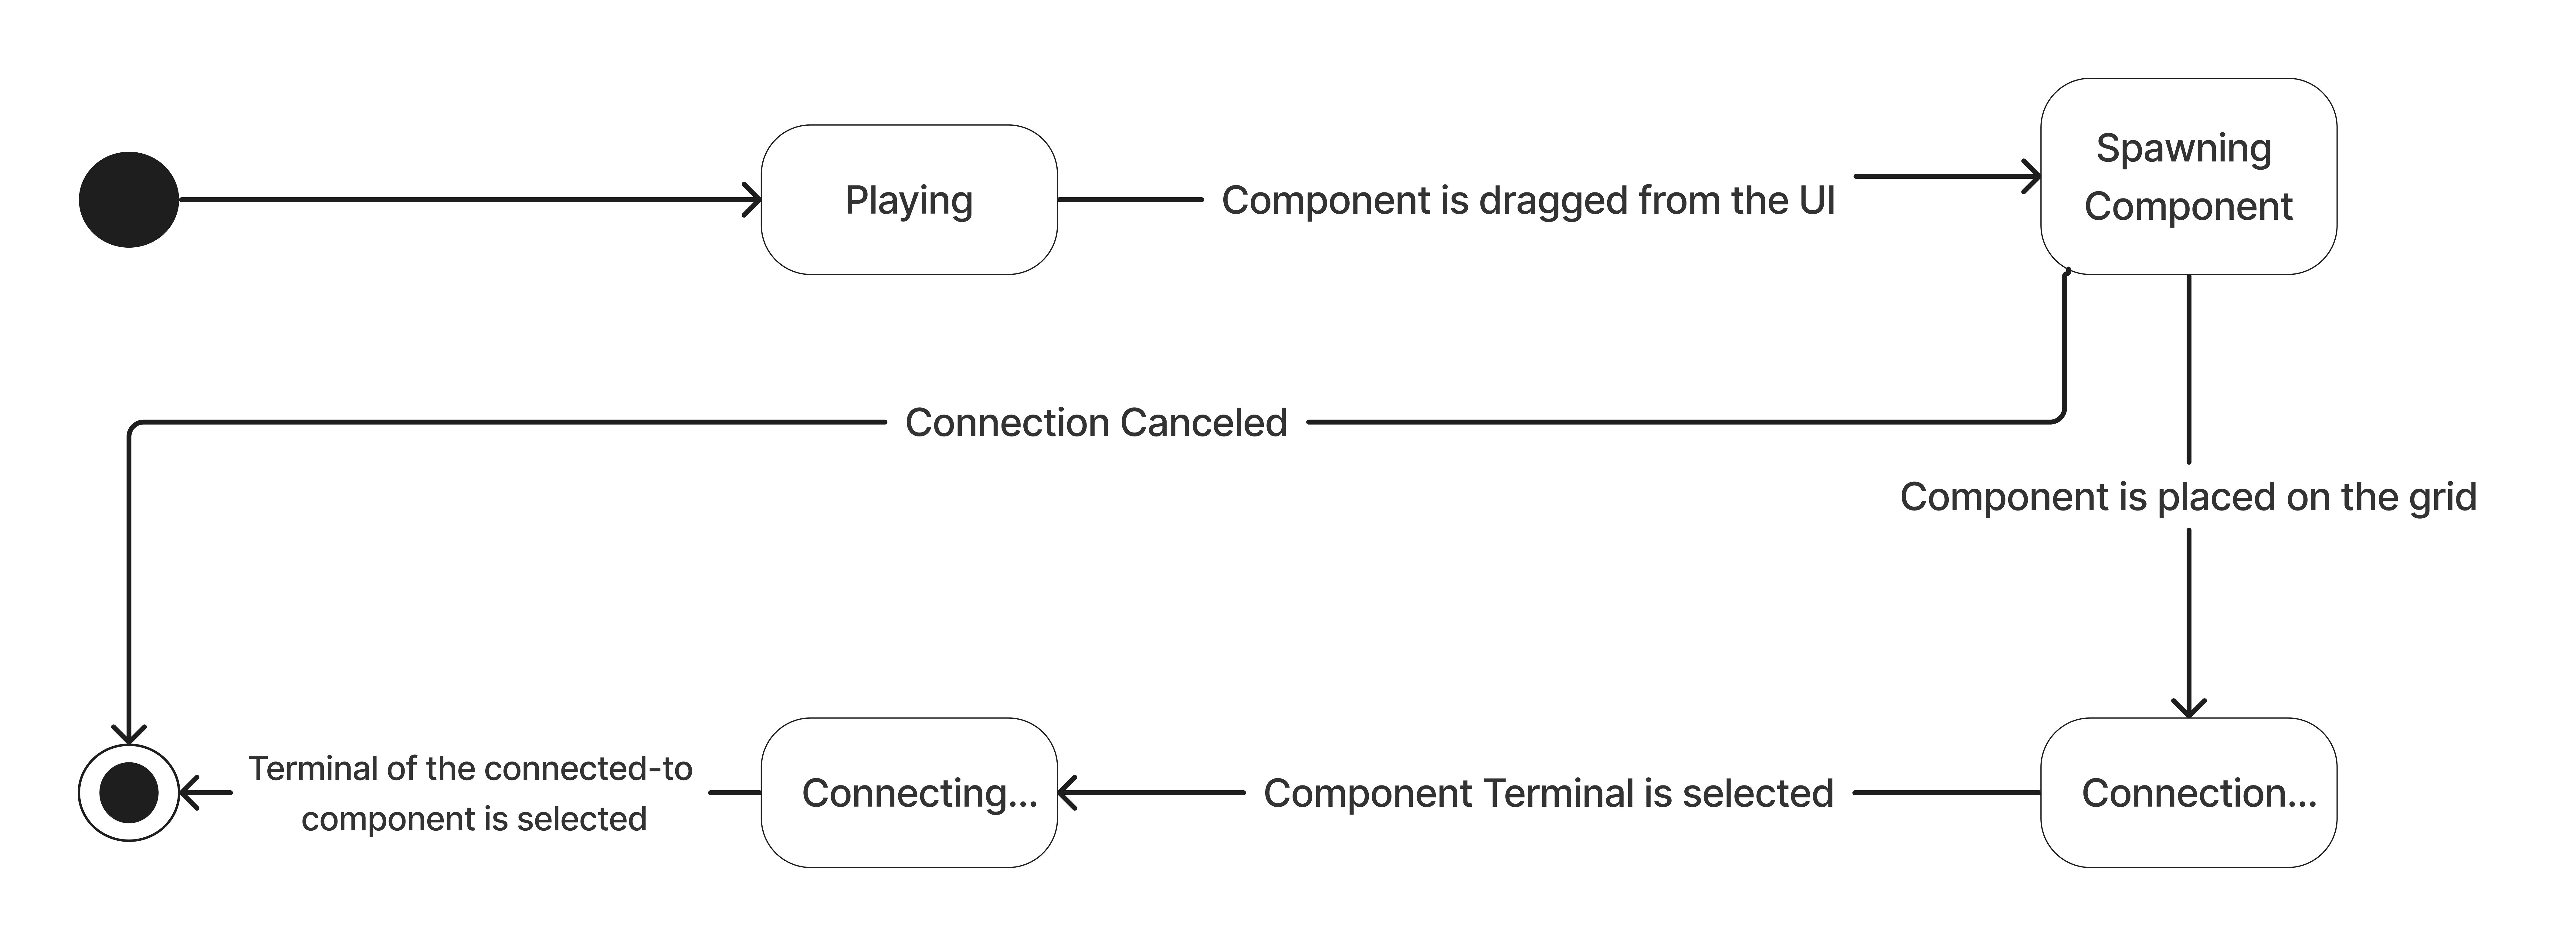
\includegraphics[scale=0.1]{images/chapter3/stateChart1.png}
\caption{Drag and Drop Components State Chart}
\label{Drag And Drop Components State Chart}
\end{figure}

\subsubsection{Simulate Circuits}
\begin{figure}[h!]
\centering
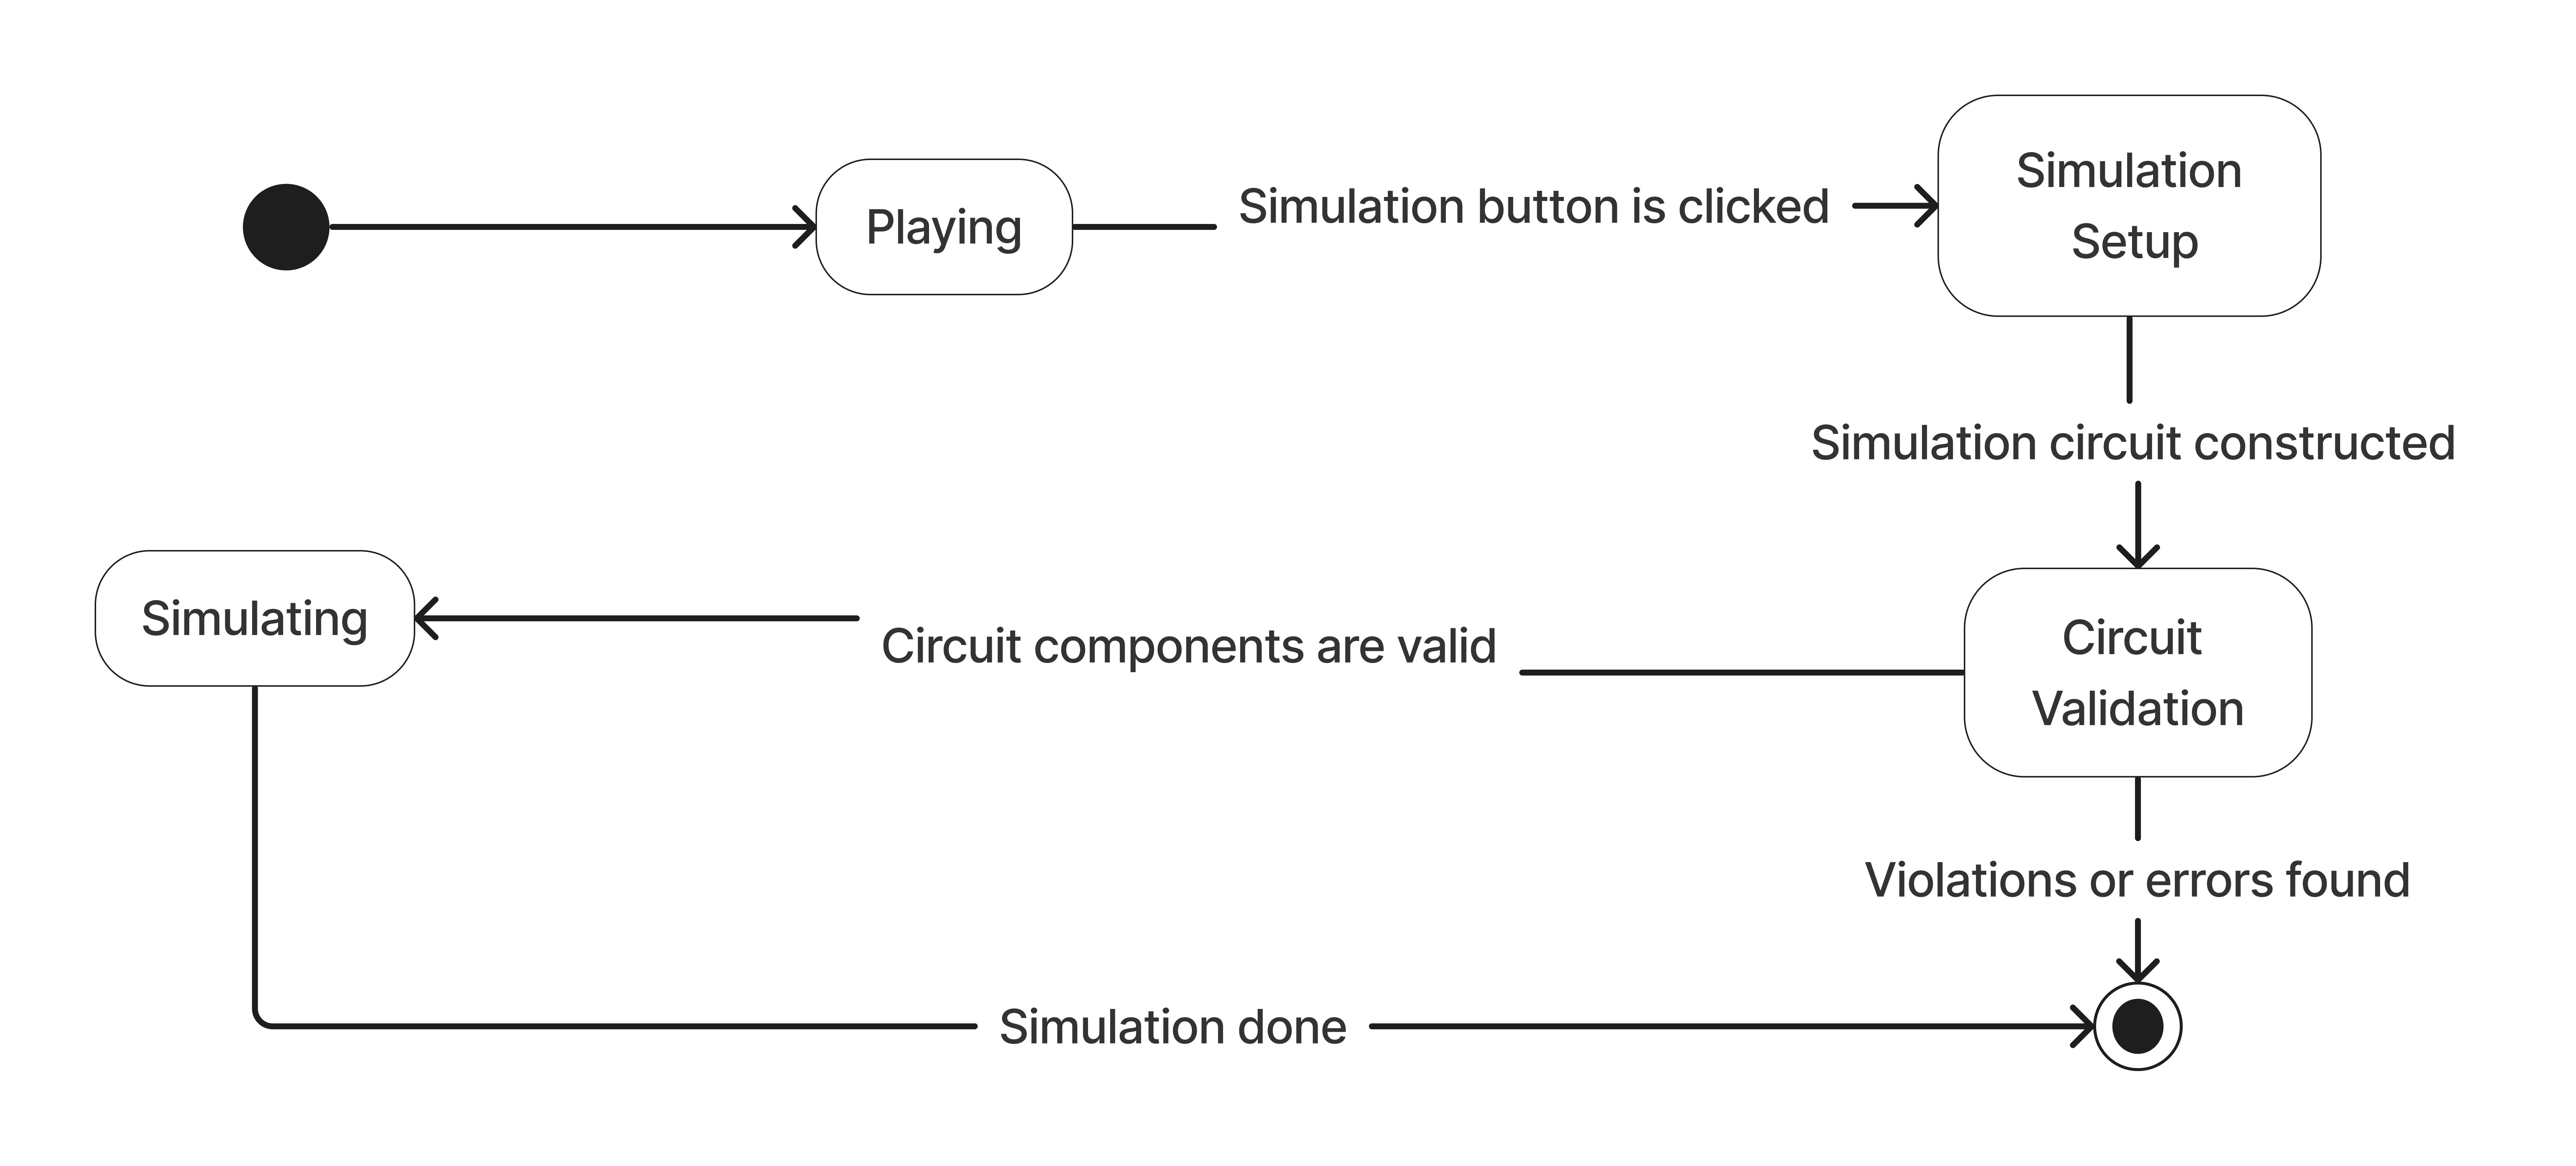
\includegraphics[scale=0.1]{images/chapter3/StateChart2.png}
\caption{Simulate Circuits State Chart}
\label{Simulate Circuits State Chart}
\end{figure}
\vfill
\newpage

\end{document}
